


% Header, overrides base

    % Make sure that the sphinx doc style knows who it inherits from.
    \def\sphinxdocclass{article}

    % Declare the document class
    \documentclass[letterpaper,10pt,english]{/usr/share/sphinx/texinputs/sphinxhowto}

    % Imports
    \usepackage[utf8]{inputenc}
    \DeclareUnicodeCharacter{00A0}{\\nobreakspace}
    \usepackage[T1]{fontenc}
    \usepackage{babel}
    \usepackage{times}
    \usepackage{import}
    \usepackage[Bjarne]{/usr/share/sphinx/texinputs/fncychap}
    \usepackage{longtable}
    \usepackage{/usr/share/sphinx/texinputs/sphinx}
    \usepackage{multirow}

    \usepackage{amsmath}
    \usepackage{amssymb}
    \usepackage{ucs}
    \usepackage{enumerate}

    % Used to make the Input/Output rules follow around the contents.
    \usepackage{needspace}

    % Pygments requirements
    \usepackage{fancyvrb}
    \usepackage{color}
    % ansi colors additions
    \definecolor{darkgreen}{rgb}{.12,.54,.11}
    \definecolor{lightgray}{gray}{.95}
    \definecolor{brown}{rgb}{0.54,0.27,0.07}
    \definecolor{purple}{rgb}{0.5,0.0,0.5}
    \definecolor{darkgray}{gray}{0.25}
    \definecolor{lightred}{rgb}{1.0,0.39,0.28}
    \definecolor{lightgreen}{rgb}{0.48,0.99,0.0}
    \definecolor{lightblue}{rgb}{0.53,0.81,0.92}
    \definecolor{lightpurple}{rgb}{0.87,0.63,0.87}
    \definecolor{lightcyan}{rgb}{0.5,1.0,0.83}

    % Needed to box output/input
    \usepackage{tikz}
        \usetikzlibrary{calc,arrows,shadows}
    \usepackage[framemethod=tikz]{mdframed}

    \usepackage{alltt}

    % Used to load and display graphics
    \usepackage{graphicx}
    \graphicspath{ {figs/} }
    \usepackage[Export]{adjustbox} % To resize

    % used so that images for notebooks which have spaces in the name can still be included
    \usepackage{grffile}


    % For formatting output while also word wrapping.
    \usepackage{listings}
    \lstset{breaklines=true}
    \lstset{basicstyle=\small\ttfamily}
    \def\smaller{\fontsize{9.5pt}{9.5pt}\selectfont}

    %Pygments definitions
    
\makeatletter
\def\PY@reset{\let\PY@it=\relax \let\PY@bf=\relax%
    \let\PY@ul=\relax \let\PY@tc=\relax%
    \let\PY@bc=\relax \let\PY@ff=\relax}
\def\PY@tok#1{\csname PY@tok@#1\endcsname}
\def\PY@toks#1+{\ifx\relax#1\empty\else%
    \PY@tok{#1}\expandafter\PY@toks\fi}
\def\PY@do#1{\PY@bc{\PY@tc{\PY@ul{%
    \PY@it{\PY@bf{\PY@ff{#1}}}}}}}
\def\PY#1#2{\PY@reset\PY@toks#1+\relax+\PY@do{#2}}

\expandafter\def\csname PY@tok@gd\endcsname{\def\PY@tc##1{\textcolor[rgb]{0.63,0.00,0.00}{##1}}}
\expandafter\def\csname PY@tok@gu\endcsname{\let\PY@bf=\textbf\def\PY@tc##1{\textcolor[rgb]{0.50,0.00,0.50}{##1}}}
\expandafter\def\csname PY@tok@gt\endcsname{\def\PY@tc##1{\textcolor[rgb]{0.00,0.27,0.87}{##1}}}
\expandafter\def\csname PY@tok@gs\endcsname{\let\PY@bf=\textbf}
\expandafter\def\csname PY@tok@gr\endcsname{\def\PY@tc##1{\textcolor[rgb]{1.00,0.00,0.00}{##1}}}
\expandafter\def\csname PY@tok@cm\endcsname{\let\PY@it=\textit\def\PY@tc##1{\textcolor[rgb]{0.25,0.50,0.50}{##1}}}
\expandafter\def\csname PY@tok@vg\endcsname{\def\PY@tc##1{\textcolor[rgb]{0.10,0.09,0.49}{##1}}}
\expandafter\def\csname PY@tok@m\endcsname{\def\PY@tc##1{\textcolor[rgb]{0.40,0.40,0.40}{##1}}}
\expandafter\def\csname PY@tok@mh\endcsname{\def\PY@tc##1{\textcolor[rgb]{0.40,0.40,0.40}{##1}}}
\expandafter\def\csname PY@tok@go\endcsname{\def\PY@tc##1{\textcolor[rgb]{0.53,0.53,0.53}{##1}}}
\expandafter\def\csname PY@tok@ge\endcsname{\let\PY@it=\textit}
\expandafter\def\csname PY@tok@vc\endcsname{\def\PY@tc##1{\textcolor[rgb]{0.10,0.09,0.49}{##1}}}
\expandafter\def\csname PY@tok@il\endcsname{\def\PY@tc##1{\textcolor[rgb]{0.40,0.40,0.40}{##1}}}
\expandafter\def\csname PY@tok@cs\endcsname{\let\PY@it=\textit\def\PY@tc##1{\textcolor[rgb]{0.25,0.50,0.50}{##1}}}
\expandafter\def\csname PY@tok@cp\endcsname{\def\PY@tc##1{\textcolor[rgb]{0.74,0.48,0.00}{##1}}}
\expandafter\def\csname PY@tok@gi\endcsname{\def\PY@tc##1{\textcolor[rgb]{0.00,0.63,0.00}{##1}}}
\expandafter\def\csname PY@tok@gh\endcsname{\let\PY@bf=\textbf\def\PY@tc##1{\textcolor[rgb]{0.00,0.00,0.50}{##1}}}
\expandafter\def\csname PY@tok@ni\endcsname{\let\PY@bf=\textbf\def\PY@tc##1{\textcolor[rgb]{0.60,0.60,0.60}{##1}}}
\expandafter\def\csname PY@tok@nl\endcsname{\def\PY@tc##1{\textcolor[rgb]{0.63,0.63,0.00}{##1}}}
\expandafter\def\csname PY@tok@nn\endcsname{\let\PY@bf=\textbf\def\PY@tc##1{\textcolor[rgb]{0.00,0.00,1.00}{##1}}}
\expandafter\def\csname PY@tok@no\endcsname{\def\PY@tc##1{\textcolor[rgb]{0.53,0.00,0.00}{##1}}}
\expandafter\def\csname PY@tok@na\endcsname{\def\PY@tc##1{\textcolor[rgb]{0.49,0.56,0.16}{##1}}}
\expandafter\def\csname PY@tok@nb\endcsname{\def\PY@tc##1{\textcolor[rgb]{0.00,0.50,0.00}{##1}}}
\expandafter\def\csname PY@tok@nc\endcsname{\let\PY@bf=\textbf\def\PY@tc##1{\textcolor[rgb]{0.00,0.00,1.00}{##1}}}
\expandafter\def\csname PY@tok@nd\endcsname{\def\PY@tc##1{\textcolor[rgb]{0.67,0.13,1.00}{##1}}}
\expandafter\def\csname PY@tok@ne\endcsname{\let\PY@bf=\textbf\def\PY@tc##1{\textcolor[rgb]{0.82,0.25,0.23}{##1}}}
\expandafter\def\csname PY@tok@nf\endcsname{\def\PY@tc##1{\textcolor[rgb]{0.00,0.00,1.00}{##1}}}
\expandafter\def\csname PY@tok@si\endcsname{\let\PY@bf=\textbf\def\PY@tc##1{\textcolor[rgb]{0.73,0.40,0.53}{##1}}}
\expandafter\def\csname PY@tok@s2\endcsname{\def\PY@tc##1{\textcolor[rgb]{0.73,0.13,0.13}{##1}}}
\expandafter\def\csname PY@tok@vi\endcsname{\def\PY@tc##1{\textcolor[rgb]{0.10,0.09,0.49}{##1}}}
\expandafter\def\csname PY@tok@nt\endcsname{\let\PY@bf=\textbf\def\PY@tc##1{\textcolor[rgb]{0.00,0.50,0.00}{##1}}}
\expandafter\def\csname PY@tok@nv\endcsname{\def\PY@tc##1{\textcolor[rgb]{0.10,0.09,0.49}{##1}}}
\expandafter\def\csname PY@tok@s1\endcsname{\def\PY@tc##1{\textcolor[rgb]{0.73,0.13,0.13}{##1}}}
\expandafter\def\csname PY@tok@sh\endcsname{\def\PY@tc##1{\textcolor[rgb]{0.73,0.13,0.13}{##1}}}
\expandafter\def\csname PY@tok@sc\endcsname{\def\PY@tc##1{\textcolor[rgb]{0.73,0.13,0.13}{##1}}}
\expandafter\def\csname PY@tok@sx\endcsname{\def\PY@tc##1{\textcolor[rgb]{0.00,0.50,0.00}{##1}}}
\expandafter\def\csname PY@tok@bp\endcsname{\def\PY@tc##1{\textcolor[rgb]{0.00,0.50,0.00}{##1}}}
\expandafter\def\csname PY@tok@c1\endcsname{\let\PY@it=\textit\def\PY@tc##1{\textcolor[rgb]{0.25,0.50,0.50}{##1}}}
\expandafter\def\csname PY@tok@kc\endcsname{\let\PY@bf=\textbf\def\PY@tc##1{\textcolor[rgb]{0.00,0.50,0.00}{##1}}}
\expandafter\def\csname PY@tok@c\endcsname{\let\PY@it=\textit\def\PY@tc##1{\textcolor[rgb]{0.25,0.50,0.50}{##1}}}
\expandafter\def\csname PY@tok@mf\endcsname{\def\PY@tc##1{\textcolor[rgb]{0.40,0.40,0.40}{##1}}}
\expandafter\def\csname PY@tok@err\endcsname{\def\PY@bc##1{\setlength{\fboxsep}{0pt}\fcolorbox[rgb]{1.00,0.00,0.00}{1,1,1}{\strut ##1}}}
\expandafter\def\csname PY@tok@kd\endcsname{\let\PY@bf=\textbf\def\PY@tc##1{\textcolor[rgb]{0.00,0.50,0.00}{##1}}}
\expandafter\def\csname PY@tok@ss\endcsname{\def\PY@tc##1{\textcolor[rgb]{0.10,0.09,0.49}{##1}}}
\expandafter\def\csname PY@tok@sr\endcsname{\def\PY@tc##1{\textcolor[rgb]{0.73,0.40,0.53}{##1}}}
\expandafter\def\csname PY@tok@mo\endcsname{\def\PY@tc##1{\textcolor[rgb]{0.40,0.40,0.40}{##1}}}
\expandafter\def\csname PY@tok@kn\endcsname{\let\PY@bf=\textbf\def\PY@tc##1{\textcolor[rgb]{0.00,0.50,0.00}{##1}}}
\expandafter\def\csname PY@tok@mi\endcsname{\def\PY@tc##1{\textcolor[rgb]{0.40,0.40,0.40}{##1}}}
\expandafter\def\csname PY@tok@gp\endcsname{\let\PY@bf=\textbf\def\PY@tc##1{\textcolor[rgb]{0.00,0.00,0.50}{##1}}}
\expandafter\def\csname PY@tok@o\endcsname{\def\PY@tc##1{\textcolor[rgb]{0.40,0.40,0.40}{##1}}}
\expandafter\def\csname PY@tok@kr\endcsname{\let\PY@bf=\textbf\def\PY@tc##1{\textcolor[rgb]{0.00,0.50,0.00}{##1}}}
\expandafter\def\csname PY@tok@s\endcsname{\def\PY@tc##1{\textcolor[rgb]{0.73,0.13,0.13}{##1}}}
\expandafter\def\csname PY@tok@kp\endcsname{\def\PY@tc##1{\textcolor[rgb]{0.00,0.50,0.00}{##1}}}
\expandafter\def\csname PY@tok@w\endcsname{\def\PY@tc##1{\textcolor[rgb]{0.73,0.73,0.73}{##1}}}
\expandafter\def\csname PY@tok@kt\endcsname{\def\PY@tc##1{\textcolor[rgb]{0.69,0.00,0.25}{##1}}}
\expandafter\def\csname PY@tok@ow\endcsname{\let\PY@bf=\textbf\def\PY@tc##1{\textcolor[rgb]{0.67,0.13,1.00}{##1}}}
\expandafter\def\csname PY@tok@sb\endcsname{\def\PY@tc##1{\textcolor[rgb]{0.73,0.13,0.13}{##1}}}
\expandafter\def\csname PY@tok@k\endcsname{\let\PY@bf=\textbf\def\PY@tc##1{\textcolor[rgb]{0.00,0.50,0.00}{##1}}}
\expandafter\def\csname PY@tok@se\endcsname{\let\PY@bf=\textbf\def\PY@tc##1{\textcolor[rgb]{0.73,0.40,0.13}{##1}}}
\expandafter\def\csname PY@tok@sd\endcsname{\let\PY@it=\textit\def\PY@tc##1{\textcolor[rgb]{0.73,0.13,0.13}{##1}}}

\def\PYZbs{\char`\\}
\def\PYZus{\char`\_}
\def\PYZob{\char`\{}
\def\PYZcb{\char`\}}
\def\PYZca{\char`\^}
\def\PYZam{\char`\&}
\def\PYZlt{\char`\<}
\def\PYZgt{\char`\>}
\def\PYZsh{\char`\#}
\def\PYZpc{\char`\%}
\def\PYZdl{\char`\$}
\def\PYZhy{\char`\-}
\def\PYZsq{\char`\'}
\def\PYZdq{\char`\"}
\def\PYZti{\char`\~}
% for compatibility with earlier versions
\def\PYZat{@}
\def\PYZlb{[}
\def\PYZrb{]}
\makeatother


    %Set pygments styles if needed...
    
        \definecolor{nbframe-border}{rgb}{0.867,0.867,0.867}
        \definecolor{nbframe-bg}{rgb}{0.969,0.969,0.969}
        \definecolor{nbframe-in-prompt}{rgb}{0.0,0.0,0.502}
        \definecolor{nbframe-out-prompt}{rgb}{0.545,0.0,0.0}

        \newenvironment{ColorVerbatim}
        {\begin{mdframed}[%
            roundcorner=1.0pt, %
            backgroundcolor=nbframe-bg, %
            userdefinedwidth=1\linewidth, %
            leftmargin=0.1\linewidth, %
            innerleftmargin=0pt, %
            innerrightmargin=0pt, %
            linecolor=nbframe-border, %
            linewidth=1pt, %
            usetwoside=false, %
            everyline=true, %
            innerlinewidth=3pt, %
            innerlinecolor=nbframe-bg, %
            middlelinewidth=1pt, %
            middlelinecolor=nbframe-bg, %
            outerlinewidth=0.5pt, %
            outerlinecolor=nbframe-border, %
            needspace=0pt
        ]}
        {\end{mdframed}}
        
        \newenvironment{InvisibleVerbatim}
        {\begin{mdframed}[leftmargin=0.1\linewidth,innerleftmargin=3pt,innerrightmargin=3pt, userdefinedwidth=1\linewidth, linewidth=0pt, linecolor=white, usetwoside=false]}
        {\end{mdframed}}

        \renewenvironment{Verbatim}[1][\unskip]
        {\begin{alltt}\smaller}
        {\end{alltt}}
    

    % Help prevent overflowing lines due to urls and other hard-to-break 
    % entities.  This doesn't catch everything...
    \sloppy

    % Document level variables
    \title{InverseVI\_uni}
    \date{October 6, 2015}
    \release{}
    \author{Unknown Author}
    \renewcommand{\releasename}{}

    % TODO: Add option for the user to specify a logo for his/her export.
    \newcommand{\sphinxlogo}{}

    % Make the index page of the document.
    \makeindex

    % Import sphinx document type specifics.
     


% Body

    % Start of the document
    \begin{document}

        
            \maketitle
        

        


        
        

    % Make sure that atleast 4 lines are below the HR
    \needspace{4\baselineskip}

    
        \vspace{6pt}
        \makebox[0.1\linewidth]{\smaller\hfill\tt\color{nbframe-in-prompt}In\hspace{4pt}{[}1{]}:\hspace{4pt}}\\*
        \vspace{-2.65\baselineskip}
        \begin{ColorVerbatim}
            \vspace{-0.7\baselineskip}
            \begin{Verbatim}[commandchars=\\\{\}]
\PY{n}{cd}\PY{p}{(}\PY{l+s}{\PYZdq{}}\PY{l+s}{/home/jzh/Dropbox/Research/Data\PYZhy{}driven\PYZus{}estimation\PYZus{}inverse\PYZus{}optimization}\PY{l+s+se}{\PYZbs{}}
\PY{l+s}{    /Experiments/InverseVIsTraffic}\PY{l+s}{\PYZdq{}}\PY{p}{)}\PY{p}{;}
\end{Verbatim}

            
                \vspace{-0.2\baselineskip}
            
        \end{ColorVerbatim}
    


    % Make sure that atleast 4 lines are below the HR
    \needspace{4\baselineskip}

    
        \vspace{6pt}
        \makebox[0.1\linewidth]{\smaller\hfill\tt\color{nbframe-in-prompt}In\hspace{4pt}{[}2{]}:\hspace{4pt}}\\*
        \vspace{-2.65\baselineskip}
        \begin{ColorVerbatim}
            \vspace{-0.7\baselineskip}
            \begin{Verbatim}[commandchars=\\\{\}]
\PY{c}{\PYZsh{}include(\PYZdq{}defArc.jl\PYZdq{})}

\PY{n+nb}{type} \PY{n}{Arc}
    \PY{n}{initNode}\PY{p}{:}\PY{p}{:}\PY{n}{Int} 
    \PY{n}{termNode}\PY{p}{:}\PY{p}{:}\PY{n}{Int} 
    \PY{n}{capacity}\PY{p}{:}\PY{p}{:}\PY{n}{Float64}
    \PY{n}{freeflowtime}\PY{p}{:}\PY{p}{:}\PY{n}{Float64}
    \PY{n}{trueflow}\PY{p}{:}\PY{p}{:}\PY{n}{Float64}
    \PY{n}{obsflow}\PY{p}{:}\PY{p}{:}\PY{n}{Float64}
\PY{n}{end}

\PY{n}{Arc}\PY{p}{(}\PY{n}{initNode}\PY{p}{:}\PY{p}{:}\PY{n}{Int}\PY{p}{,} \PY{n}{termNode}\PY{p}{:}\PY{p}{:}\PY{n}{Int}\PY{p}{,} \PY{n}{capacity}\PY{p}{:}\PY{p}{:}\PY{n}{Float64}\PY{p}{,}\PYZbs{}
    \PY{n}{freeflowtime}\PY{p}{:}\PY{p}{:}\PY{n}{Float64}\PY{p}{)} \PY{o}{=} 
    \PY{n}{Arc}\PY{p}{(}\PY{n}{initNode}\PY{p}{,} \PY{n}{termNode}\PY{p}{,} \PY{n}{capacity}\PY{p}{,} \PY{n}{freeflowtime}\PY{p}{,} \PY{l+m+mf}{0.}\PY{p}{,} \PY{l+m+mf}{0.}\PY{p}{)}
\end{Verbatim}

            
                \vspace{-0.2\baselineskip}
            
        \end{ColorVerbatim}
    

    

        % If the first block is an image, minipage the image.  Else
        % request a certain amount of space for the input text.
        \needspace{4\baselineskip}
        
        

            % Add document contents.
            
                \makebox[0.1\linewidth]{\smaller\hfill\tt\color{nbframe-out-prompt}Out\hspace{4pt}{[}2{]}:\hspace{4pt}}\\*
                \vspace{-2.55\baselineskip}\begin{InvisibleVerbatim}
                \vspace{-0.5\baselineskip}
\begin{alltt}Arc (constructor with 3 methods)\end{alltt}

            \end{InvisibleVerbatim}
            
        
    


    % Make sure that atleast 4 lines are below the HR
    \needspace{4\baselineskip}

    
        \vspace{6pt}
        \makebox[0.1\linewidth]{\smaller\hfill\tt\color{nbframe-in-prompt}In\hspace{4pt}{[}3{]}:\hspace{4pt}}\\*
        \vspace{-2.65\baselineskip}
        \begin{ColorVerbatim}
            \vspace{-0.7\baselineskip}
            \begin{Verbatim}[commandchars=\\\{\}]
\PY{c}{\PYZsh{}include(\PYZdq{}fitTraffic.jl\PYZdq{})}

\PY{c}{\PYZsh{}\PYZsh{} Solve an inverse tarffic problem over polynomials }
\PY{c}{\PYZsh{}\PYZsh{} of degree at most d}
\PY{c}{\PYZsh{}\PYZsh{} optionally use a regularizer from the poly kernel}

\PY{n}{using} \PY{n}{JuMP}
\PY{n}{using} \PY{n}{Gurobi}
\PY{n}{using} \PY{n}{Graphs}
\PY{n}{using} \PY{n}{Roots}


\PY{n}{polyEval}\PY{p}{(}\PY{n}{coeffs}\PY{p}{,} \PY{n}{pt}\PY{p}{)} \PY{o}{=} \PY{n+nb}{sum}\PY{p}{(}\PY{p}{[}\PY{n}{coeffs}\PY{p}{[}\PY{n}{i}\PY{p}{]} \PY{o}{*} \PY{n}{pt}\PY{o}{\PYZca{}}\PY{p}{(}\PY{n}{i}\PY{o}{\PYZhy{}}\PY{l+m+mi}{1}\PY{p}{)} \PYZbs{}
                            \PY{k}{for} \PY{n}{i} \PY{o}{=} \PY{l+m+mi}{1}\PY{p}{:}\PY{n}{length}\PY{p}{(}\PY{n}{coeffs}\PY{p}{)}\PY{p}{]}\PY{p}{)}  
\PY{c}{\PYZsh{}VG think about faster way to do this}

\PY{n}{polyEval}\PY{p}{(}\PY{n}{coeffs}\PY{p}{:}\PY{p}{:}\PY{n}{Array}\PY{p}{\PYZob{}}\PY{n}{Float64}\PY{p}{,} \PY{l+m+mi}{1}\PY{p}{\PYZcb{}}\PY{p}{,} \PY{n}{pt}\PY{p}{)} \PY{o}{=} \PYZbs{}
    \PY{n+nb}{sum}\PY{p}{(}\PY{p}{[}\PY{n}{coeffs}\PY{p}{[}\PY{n}{i}\PY{p}{]} \PY{o}{*} \PY{n}{pt}\PY{o}{\PYZca{}}\PY{p}{(}\PY{n}{i}\PY{o}{\PYZhy{}}\PY{l+m+mi}{1}\PY{p}{)} \PY{k}{for} \PY{n}{i} \PY{o}{=} \PY{l+m+mi}{1}\PY{p}{:}\PY{n}{length}\PY{p}{(}\PY{n}{coeffs}\PY{p}{)}\PY{p}{]}\PY{p}{)} 
    \PY{c}{\PYZsh{}separate for consts}

\PY{n}{bpacost}\PY{p}{(}\PY{n}{flow}\PY{p}{:}\PY{p}{:}\PY{n}{Float64}\PY{p}{,} \PY{n}{capacity}\PY{p}{:}\PY{p}{:}\PY{n}{Float64}\PY{p}{,} \PY{n}{freeflowtime}\PY{p}{:}\PY{p}{:}\PY{n}{Float64}\PY{p}{)} \PYZbs{}
        \PY{o}{=} \PY{n}{freeflowtime}\PY{o}{*}\PY{p}{(}\PY{l+m+mi}{1} \PY{o}{+} \PY{o}{.}\PY{l+m+mi}{15} \PY{o}{*} \PY{p}{(}\PY{n}{flow}\PY{o}{/}\PY{n}{capacity}\PY{p}{)}\PY{o}{\PYZca{}}\PY{l+m+mi}{4}\PY{p}{)}
\PY{n}{bpacost}\PY{p}{(}\PY{n}{flow}\PY{p}{:}\PY{p}{:}\PY{n}{Float64}\PY{p}{,} \PY{n}{arc}\PY{p}{)} \PY{o}{=} \PY{n}{bpacost}\PY{p}{(}\PY{n}{flow}\PY{p}{,} \PY{n}{arc}\PY{o}{.}\PY{n}{capacity}\PY{p}{,} \PY{n}{arc}\PY{o}{.}\PY{n}{freeflowtime}\PY{p}{)}
\PY{n}{bpacost}\PY{p}{(}\PY{n}{arc}\PY{p}{:}\PY{p}{:}\PY{n}{Arc}\PY{p}{)} \PY{o}{=} \PY{n}{bpacost}\PY{p}{(}\PY{n}{arc}\PY{o}{.}\PY{n}{obsflow}\PY{p}{,} \PY{n}{arc}\PY{p}{)}
\end{Verbatim}

            
                \vspace{-0.2\baselineskip}
            
        \end{ColorVerbatim}
    

    

        % If the first block is an image, minipage the image.  Else
        % request a certain amount of space for the input text.
        \needspace{4\baselineskip}
        
        

            % Add document contents.
            
                \makebox[0.1\linewidth]{\smaller\hfill\tt\color{nbframe-out-prompt}Out\hspace{4pt}{[}3{]}:\hspace{4pt}}\\*
                \vspace{-2.55\baselineskip}\begin{InvisibleVerbatim}
                \vspace{-0.5\baselineskip}
\begin{alltt}bpacost (generic function with 3 methods)\end{alltt}

            \end{InvisibleVerbatim}
            
        
    


    % Make sure that atleast 4 lines are below the HR
    \needspace{4\baselineskip}

    
        \vspace{6pt}
        \makebox[0.1\linewidth]{\smaller\hfill\tt\color{nbframe-in-prompt}In\hspace{4pt}{[}4{]}:\hspace{4pt}}\\*
        \vspace{-2.65\baselineskip}
        \begin{ColorVerbatim}
            \vspace{-0.7\baselineskip}
            \begin{Verbatim}[commandchars=\\\{\}]
\PY{n}{function} \PY{n}{setUpFitting}\PY{p}{(}\PY{n}{deg}\PY{p}{:}\PY{p}{:}\PY{n}{Int}\PY{p}{,} \PY{n}{c}\PY{p}{,} \PY{n}{odpairs}\PY{p}{,} \PY{n}{nodes}\PY{p}{)}
	\PY{n}{m} \PY{o}{=} \PY{n}{Model}\PY{p}{(}\PY{n}{solver}\PY{o}{=}\PY{n}{GurobiSolver}\PY{p}{(}\PY{n}{OutputFlag}\PY{o}{=}\PY{n}{false}\PY{p}{)}\PY{p}{)}
	\PY{n+nd}{@defVar}\PY{p}{(}\PY{n}{m}\PY{p}{,} \PY{n}{coeffs}\PY{p}{[}\PY{l+m+mi}{1}\PY{p}{:}\PY{n}{deg}\PY{o}{+}\PY{l+m+mi}{1}\PY{p}{]}\PY{p}{)}
	\PY{n+nd}{@defVar}\PY{p}{(}\PY{n}{m}\PY{p}{,} \PY{n}{Calphas}\PY{p}{[}\PY{l+m+mi}{1}\PY{p}{:}\PY{n}{deg}\PY{o}{+}\PY{l+m+mi}{1}\PY{p}{]}\PY{p}{)}

	\PY{c}{\PYZsh{}\PYZsh{}VG Probably want to go back and redo this with an intercept term}
	\PY{c}{\PYZsh{}build the graham matrix}
	\PY{n}{samples} \PY{o}{=} \PY{n}{linspace}\PY{p}{(}\PY{l+m+mi}{0}\PY{p}{,} \PY{l+m+mi}{1}\PY{p}{,} \PY{n}{deg} \PY{o}{+} \PY{l+m+mi}{1}\PY{p}{)}
	\PY{n}{k}\PY{p}{(}\PY{n}{x}\PY{p}{,}\PY{n}{y}\PY{p}{)} \PY{o}{=} \PY{p}{(}\PY{n}{c} \PY{o}{+} \PY{n}{x}\PY{o}{*}\PY{n}{y}\PY{p}{)}\PY{o}{\PYZca{}}\PY{n}{deg}
	\PY{n}{K} \PY{o}{=} \PY{p}{[} \PY{n}{k}\PY{p}{(}\PY{n}{x}\PY{p}{,}\PY{n}{y}\PY{p}{)} \PY{k}{for} \PY{n}{x} \PY{o}{=} \PY{n}{samples}\PY{p}{,} \PY{n}{y}\PY{o}{=}\PY{n}{samples}\PY{p}{]}
	\PY{n}{K} \PY{o}{=} \PY{n}{convert}\PY{p}{(}\PY{n}{Array}\PY{p}{\PYZob{}}\PY{n}{Float64}\PY{p}{,} \PY{l+m+mi}{2}\PY{p}{\PYZcb{}}\PY{p}{,} \PY{n}{K}\PY{p}{)}
	\PY{k}{assert}\PY{p}{(}\PY{n}{rank}\PY{p}{(}\PY{n}{K}\PY{p}{)} \PY{o}{==} \PY{n}{deg}\PY{o}{+}\PY{l+m+mi}{1}\PY{p}{)}
	\PY{n}{C} \PY{o}{=} \PY{n}{chol}\PY{p}{(}\PY{n}{K} \PY{o}{+} \PY{l+m+mf}{1e\PYZhy{}6}\PY{o}{*} \PY{n}{eye}\PY{p}{(}\PY{n}{deg}\PY{o}{+}\PY{l+m+mi}{1}\PY{p}{)}\PY{p}{)}
	\PY{k}{for} \PY{n}{i}\PY{o}{=}\PY{l+m+mi}{1}\PY{p}{:}\PY{n}{deg} \PY{o}{+} \PY{l+m+mi}{1}
		\PY{n+nd}{@addConstraint}\PY{p}{(}\PY{n}{m}\PY{p}{,} \PY{n}{polyEval}\PY{p}{(}\PY{n}{coeffs}\PY{p}{,} \PY{n}{samples}\PY{p}{[}\PY{n}{i}\PY{p}{]}\PY{p}{)} \PY{o}{==} 
						\PY{n+nb}{sum}\PY{p}{\PYZob{}}\PY{n}{C}\PY{p}{[}\PY{n}{j}\PY{p}{,} \PY{n}{i}\PY{p}{]} \PY{o}{*} \PY{n}{Calphas}\PY{p}{[}\PY{n}{j}\PY{p}{]}\PY{p}{,} \PY{n}{j}\PY{o}{=}\PY{l+m+mi}{1}\PY{p}{:}\PY{n}{deg}\PY{o}{+}\PY{l+m+mi}{1}\PY{p}{\PYZcb{}}\PY{p}{)}
	\PY{n}{end}
	\PY{n+nd}{@defVar}\PY{p}{(}\PY{n}{m}\PY{p}{,} \PY{n}{reg\PYZus{}term} \PY{o}{\PYZgt{}}\PY{o}{=} \PY{l+m+mi}{0}\PY{p}{)}
	\PY{n}{reg\PYZus{}term\PYZus{}} \PY{o}{=} \PY{n}{QuadExpr}\PY{p}{(}\PY{n}{Calphas}\PY{p}{[}\PY{p}{:}\PY{p}{]}\PY{p}{,} \PY{n}{Calphas}\PY{p}{[}\PY{p}{:}\PY{p}{]}\PY{p}{,} \PY{n}{ones}\PY{p}{(}\PY{n}{deg}\PY{o}{+}\PY{l+m+mi}{1}\PY{p}{)}\PY{p}{,} \PY{n}{AffExpr}\PY{p}{(}\PY{p}{)} \PY{p}{)}
	\PY{n+nd}{@addConstraint}\PY{p}{(}\PY{n}{m}\PY{p}{,} \PY{n}{reg\PYZus{}term} \PY{o}{\PYZgt{}}\PY{o}{=} \PY{n}{reg\PYZus{}term\PYZus{}}\PY{p}{)}

	\PY{k}{return} \PY{n}{m}\PY{p}{,} \PY{n}{coeffs}\PY{p}{,} \PY{n}{reg\PYZus{}term}
\PY{n}{end}
\end{Verbatim}

            
                \vspace{-0.2\baselineskip}
            
        \end{ColorVerbatim}
    

    

        % If the first block is an image, minipage the image.  Else
        % request a certain amount of space for the input text.
        \needspace{4\baselineskip}
        
        

            % Add document contents.
            
                \makebox[0.1\linewidth]{\smaller\hfill\tt\color{nbframe-out-prompt}Out\hspace{4pt}{[}4{]}:\hspace{4pt}}\\*
                \vspace{-2.55\baselineskip}\begin{InvisibleVerbatim}
                \vspace{-0.5\baselineskip}
\begin{alltt}setUpFitting (generic function with 1 method)\end{alltt}

            \end{InvisibleVerbatim}
            
        
    


    % Make sure that atleast 4 lines are below the HR
    \needspace{4\baselineskip}

    
        \vspace{6pt}
        \makebox[0.1\linewidth]{\smaller\hfill\tt\color{nbframe-in-prompt}In\hspace{4pt}{[}5{]}:\hspace{4pt}}\\*
        \vspace{-2.65\baselineskip}
        \begin{ColorVerbatim}
            \vspace{-0.7\baselineskip}
            \begin{Verbatim}[commandchars=\\\{\}]
\PY{n}{function} \PY{n}{fixCoeffs}\PY{p}{(}\PY{n}{m}\PY{p}{,} \PY{n}{fcoeffs}\PY{p}{,} \PY{n}{coeffs}\PY{p}{)}
	\PY{k}{for} \PY{p}{(}\PY{n}{fc}\PY{p}{,} \PY{n}{c}\PY{p}{)} \PY{o+ow}{in} \PY{n+nb}{zip}\PY{p}{(}\PY{n}{fcoeffs}\PY{p}{,} \PY{n}{coeffs}\PY{p}{[}\PY{p}{:}\PY{p}{]}\PY{p}{)}
		\PY{n+nd}{@addConstraint}\PY{p}{(}\PY{n}{m}\PY{p}{,} \PY{n}{fc} \PY{o}{==} \PY{n}{c}\PY{p}{)}
	\PY{n}{end}
\PY{n}{end}
\end{Verbatim}

            
                \vspace{-0.2\baselineskip}
            
        \end{ColorVerbatim}
    

    

        % If the first block is an image, minipage the image.  Else
        % request a certain amount of space for the input text.
        \needspace{4\baselineskip}
        
        

            % Add document contents.
            
                \makebox[0.1\linewidth]{\smaller\hfill\tt\color{nbframe-out-prompt}Out\hspace{4pt}{[}5{]}:\hspace{4pt}}\\*
                \vspace{-2.55\baselineskip}\begin{InvisibleVerbatim}
                \vspace{-0.5\baselineskip}
\begin{alltt}fixCoeffs (generic function with 1 method)\end{alltt}

            \end{InvisibleVerbatim}
            
        
    


    % Make sure that atleast 4 lines are below the HR
    \needspace{4\baselineskip}

    
        \vspace{6pt}
        \makebox[0.1\linewidth]{\smaller\hfill\tt\color{nbframe-in-prompt}In\hspace{4pt}{[}6{]}:\hspace{4pt}}\\*
        \vspace{-2.65\baselineskip}
        \begin{ColorVerbatim}
            \vspace{-0.7\baselineskip}
            \begin{Verbatim}[commandchars=\\\{\}]
\PY{n}{function} \PY{n}{addResid}\PY{p}{(}\PY{n}{m}\PY{p}{,} \PY{n}{coeffs}\PY{p}{,} \PY{n}{ys}\PY{p}{,} \PY{n}{demands}\PY{p}{,} \PY{n}{arcs}\PY{p}{,} \PY{n}{scaling}\PY{p}{)}
	\PY{n+nd}{@defVar}\PY{p}{(}\PY{n}{m}\PY{p}{,} \PY{n}{resid}\PY{p}{)}
	\PY{n+nd}{@defVar}\PY{p}{(}\PY{n}{m}\PY{p}{,} \PY{n}{dual\PYZus{}cost}\PY{p}{)}
	\PY{n+nd}{@defVar}\PY{p}{(}\PY{n}{m}\PY{p}{,} \PY{n}{primal\PYZus{}cost}\PY{p}{)}

	\PY{n+nd}{@addConstraint}\PY{p}{(}\PY{n}{m}\PY{p}{,} \PY{n}{dual\PYZus{}cost} \PY{o}{==} \PY{n+nb}{sum}\PY{p}{\PYZob{}}\PY{n}{demands}\PY{p}{[}\PY{p}{(}\PY{n}{s}\PY{p}{,}\PY{n}{t}\PY{p}{)}\PY{p}{]} \PY{o}{*} \PYZbs{}
                \PY{p}{(}\PY{n}{ys}\PY{p}{[}\PY{p}{(}\PY{n}{s}\PY{p}{,}\PY{n}{t}\PY{p}{)}\PY{p}{,} \PY{n}{t}\PY{p}{]} \PY{o}{\PYZhy{}} \PY{n}{ys}\PY{p}{[}\PY{p}{(}\PY{n}{s}\PY{p}{,}\PY{n}{t}\PY{p}{)}\PY{p}{,} \PY{n}{s}\PY{p}{]}\PY{p}{)}\PY{p}{,} \PY{p}{(}\PY{n}{s}\PY{p}{,}\PY{n}{t}\PY{p}{)}\PY{o}{=}\PY{n}{keys}\PY{p}{(}\PY{n}{demands}\PY{p}{)}\PY{p}{\PYZcb{}}\PY{p}{)}  
	\PY{n+nd}{@addConstraint}\PY{p}{(}\PY{n}{m}\PY{p}{,} \PY{n}{primal\PYZus{}cost} \PY{o}{==} \PY{n+nb}{sum}\PY{p}{\PYZob{}}\PY{n}{a}\PY{o}{.}\PY{n}{obsflow} \PY{o}{*} \PY{n}{a}\PY{o}{.}\PY{n}{freeflowtime} \PY{o}{*} 
            \PY{n}{polyEval}\PY{p}{(}\PY{n}{coeffs}\PY{p}{,} \PY{n}{a}\PY{o}{.}\PY{n}{obsflow}\PY{o}{/}\PY{n}{a}\PY{o}{.}\PY{n}{capacity}\PY{p}{)}\PY{p}{,} \PY{n}{a}\PY{o}{=}\PY{n}{values}\PY{p}{(}\PY{n}{arcs}\PY{p}{)}\PY{p}{\PYZcb{}}\PY{p}{)}

	\PY{n+nd}{@addConstraint}\PY{p}{(}\PY{n}{m}\PY{p}{,} \PY{n}{resid} \PY{o}{\PYZgt{}}\PY{o}{=} \PY{p}{(}\PY{n}{dual\PYZus{}cost} \PY{o}{\PYZhy{}} \PY{n}{primal\PYZus{}cost}\PY{p}{)} \PY{o}{/} \PY{n}{scaling} \PY{p}{)}
	\PY{n+nd}{@addConstraint}\PY{p}{(}\PY{n}{m}\PY{p}{,} \PY{n}{resid} \PY{o}{\PYZgt{}}\PY{o}{=} \PY{p}{(}\PY{n}{primal\PYZus{}cost} \PY{o}{\PYZhy{}} \PY{n}{dual\PYZus{}cost}\PY{p}{)} \PY{o}{/} \PY{n}{scaling} \PY{p}{)}
	\PY{k}{return} \PY{n}{resid}
\PY{n}{end}
\end{Verbatim}

            
                \vspace{-0.2\baselineskip}
            
        \end{ColorVerbatim}
    

    

        % If the first block is an image, minipage the image.  Else
        % request a certain amount of space for the input text.
        \needspace{4\baselineskip}
        
        

            % Add document contents.
            
                \makebox[0.1\linewidth]{\smaller\hfill\tt\color{nbframe-out-prompt}Out\hspace{4pt}{[}6{]}:\hspace{4pt}}\\*
                \vspace{-2.55\baselineskip}\begin{InvisibleVerbatim}
                \vspace{-0.5\baselineskip}
\begin{alltt}addResid (generic function with 1 method)\end{alltt}

            \end{InvisibleVerbatim}
            
        
    


    % Make sure that atleast 4 lines are below the HR
    \needspace{4\baselineskip}

    
        \vspace{6pt}
        \makebox[0.1\linewidth]{\smaller\hfill\tt\color{nbframe-in-prompt}In\hspace{4pt}{[}7{]}:\hspace{4pt}}\\*
        \vspace{-2.65\baselineskip}
        \begin{ColorVerbatim}
            \vspace{-0.7\baselineskip}
            \begin{Verbatim}[commandchars=\\\{\}]
\PY{n}{function} \PY{n}{addIncreasingCnsts}\PY{p}{(}\PY{n}{m}\PY{p}{,} \PY{n}{coeffs}\PY{p}{,} \PY{n}{arcs}\PY{p}{;} \PY{n}{TOL}\PY{o}{=}\PY{l+m+mf}{0.}\PY{p}{)}
	\PY{n}{sorted\PYZus{}flows} \PY{o}{=} \PY{n}{sort}\PY{p}{(}\PY{p}{[}\PY{n}{a}\PY{o}{.}\PY{n}{obsflow} \PY{o}{/} \PY{n}{a}\PY{o}{.}\PY{n}{capacity} \PY{k}{for} \PY{n}{a} \PY{o+ow}{in} \PY{n}{values}\PY{p}{(}\PY{n}{arcs}\PY{p}{)}\PY{p}{]}\PY{p}{)}
	\PY{n+nd}{@addConstraint}\PY{p}{(}\PY{n}{m}\PY{p}{,} \PY{n}{polyEval}\PY{p}{(}\PY{n}{coeffs}\PY{p}{,} \PY{l+m+mi}{0}\PY{p}{)} \PY{o}{\PYZlt{}}\PY{o}{=} \PYZbs{}
                   \PY{n}{polyEval}\PY{p}{(}\PY{n}{coeffs}\PY{p}{,} \PY{n}{sorted\PYZus{}flows}\PY{p}{[}\PY{l+m+mi}{1}\PY{p}{]}\PY{p}{)}\PY{p}{)}
	\PY{k}{for} \PY{n}{i} \PY{o}{=} \PY{l+m+mi}{2}\PY{p}{:}\PY{n}{length}\PY{p}{(}\PY{n}{sorted\PYZus{}flows}\PY{p}{)}
		\PY{n+nd}{@addConstraint}\PY{p}{(}\PY{n}{m}\PY{p}{,} \PY{n}{polyEval}\PY{p}{(}\PY{n}{coeffs}\PY{p}{,} \PY{n}{sorted\PYZus{}flows}\PY{p}{[}\PY{n}{i}\PY{o}{\PYZhy{}}\PY{l+m+mi}{1}\PY{p}{]}\PY{p}{)} \PYZbs{}
                       \PY{o}{\PYZlt{}}\PY{o}{=} \PY{n}{polyEval}\PY{p}{(}\PY{n}{coeffs}\PY{p}{,} \PY{n}{sorted\PYZus{}flows}\PY{p}{[}\PY{n}{i}\PY{p}{]}\PY{p}{)} \PY{o}{+} \PY{n}{TOL}\PY{p}{)}
	\PY{n}{end}
\PY{n}{end}
\end{Verbatim}

            
                \vspace{-0.2\baselineskip}
            
        \end{ColorVerbatim}
    

    

        % If the first block is an image, minipage the image.  Else
        % request a certain amount of space for the input text.
        \needspace{4\baselineskip}
        
        

            % Add document contents.
            
                \makebox[0.1\linewidth]{\smaller\hfill\tt\color{nbframe-out-prompt}Out\hspace{4pt}{[}7{]}:\hspace{4pt}}\\*
                \vspace{-2.55\baselineskip}\begin{InvisibleVerbatim}
                \vspace{-0.5\baselineskip}
\begin{alltt}addIncreasingCnsts (generic function with 1 method)\end{alltt}

            \end{InvisibleVerbatim}
            
        
    


    % Make sure that atleast 4 lines are below the HR
    \needspace{4\baselineskip}

    
        \vspace{6pt}
        \makebox[0.1\linewidth]{\smaller\hfill\tt\color{nbframe-in-prompt}In\hspace{4pt}{[}8{]}:\hspace{4pt}}\\*
        \vspace{-2.65\baselineskip}
        \begin{ColorVerbatim}
            \vspace{-0.7\baselineskip}
            \begin{Verbatim}[commandchars=\\\{\}]
\PY{c}{\PYZsh{}equates the total cost of the network to the true total cost}
\PY{n}{function} \PY{n}{normalize}\PY{p}{(}\PY{n}{m}\PY{p}{,} \PY{n}{coeffs}\PY{p}{,} \PY{n}{tot\PYZus{}true\PYZus{}cost}\PY{p}{:}\PY{p}{:}\PY{n}{Float64}\PY{p}{,} \PY{n}{arcs}\PY{p}{)}
	\PY{n+nd}{@addConstraint}\PY{p}{(}\PY{n}{m}\PY{p}{,} 
		\PY{n+nb}{sum}\PY{p}{\PYZob{}}\PY{n}{a}\PY{o}{.}\PY{n}{freeflowtime} \PY{o}{*} \PY{n}{a}\PY{o}{.}\PY{n}{obsflow} \PY{o}{*} \PYZbs{}
            \PY{n}{polyEval}\PY{p}{(}\PY{n}{coeffs}\PY{p}{,} \PY{n}{a}\PY{o}{.}\PY{n}{obsflow} \PY{o}{/} \PY{n}{a}\PY{o}{.}\PY{n}{capacity}\PY{p}{)}\PY{p}{,} 
			\PY{n}{a}\PY{o}{=}\PY{n}{values}\PY{p}{(}\PY{n}{arcs}\PY{p}{)}\PY{p}{\PYZcb{}} \PY{o}{==} \PY{n}{tot\PYZus{}true\PYZus{}cost}\PY{p}{)}
\PY{n}{end}

\PY{n}{function} \PY{n}{normalize}\PY{p}{(}\PY{n}{m}\PY{p}{,} \PY{n}{coeffs}\PY{p}{,} \PY{n}{scaled\PYZus{}flow}\PY{p}{:}\PY{p}{:}\PY{n}{Float64}\PY{p}{,} \PY{n}{cost}\PY{p}{:}\PY{p}{:}\PY{n}{Float64}\PY{p}{)}
	\PY{n+nd}{@addConstraint}\PY{p}{(}\PY{n}{m}\PY{p}{,} \PY{n}{polyEval}\PY{p}{(}\PY{n}{coeffs}\PY{p}{,} \PY{n}{scaled\PYZus{}flow}\PY{p}{)} \PY{o}{==} \PY{n}{cost}\PY{p}{)}
\PY{n}{end}

\PY{n}{function} \PY{n}{normalize}\PY{p}{(}\PY{n}{m}\PY{p}{,} \PY{n}{coeffs}\PY{p}{,} \PY{n}{scaled\PYZus{}flows}\PY{p}{:}\PY{p}{:}\PY{n}{Array}\PY{p}{\PYZob{}}\PY{n}{Float64}\PY{p}{,} \PY{l+m+mi}{1}\PY{p}{\PYZcb{}}\PY{p}{,} \PYZbs{}
                   \PY{n}{avgCost}\PY{p}{:}\PY{p}{:}\PY{n}{Float64}\PY{p}{)}
    \PY{n+nd}{@addConstraint}\PY{p}{(}\PY{n}{m}\PY{p}{,} \PY{n+nb}{sum}\PY{p}{\PYZob{}}\PY{n}{polyEval}\PY{p}{(}\PY{n}{coeffs}\PY{p}{,} \PY{n}{f}\PY{p}{)}\PY{p}{,} \PY{n}{f}\PY{o}{=}\PY{n}{scaled\PYZus{}flows}\PY{p}{\PYZcb{}} \PYZbs{}
                   \PY{o}{==} \PY{n}{avgCost} \PY{o}{*} \PY{n}{length}\PY{p}{(}\PY{n}{scaled\PYZus{}flows}\PY{p}{)}\PY{p}{)}
\PY{n}{end}
\end{Verbatim}

            
                \vspace{-0.2\baselineskip}
            
        \end{ColorVerbatim}
    

    

        % If the first block is an image, minipage the image.  Else
        % request a certain amount of space for the input text.
        \needspace{4\baselineskip}
        
        

            % Add document contents.
            
                \makebox[0.1\linewidth]{\smaller\hfill\tt\color{nbframe-out-prompt}Out\hspace{4pt}{[}8{]}:\hspace{4pt}}\\*
                \vspace{-2.55\baselineskip}\begin{InvisibleVerbatim}
                \vspace{-0.5\baselineskip}
\begin{alltt}normalize (generic function with 3 methods)\end{alltt}

            \end{InvisibleVerbatim}
            
        
    


    % Make sure that atleast 4 lines are below the HR
    \needspace{4\baselineskip}

    
        \vspace{6pt}
        \makebox[0.1\linewidth]{\smaller\hfill\tt\color{nbframe-in-prompt}In\hspace{4pt}{[}9{]}:\hspace{4pt}}\\*
        \vspace{-2.65\baselineskip}
        \begin{ColorVerbatim}
            \vspace{-0.7\baselineskip}
            \begin{Verbatim}[commandchars=\\\{\}]
\PY{n}{function} \PY{n}{addNetworkCnsts}\PY{p}{(}\PY{n}{m}\PY{p}{,} \PY{n}{coeffs}\PY{p}{,} \PY{n}{demands}\PY{p}{,} \PY{n}{arcs}\PY{p}{,} \PY{n}{numNodes}\PY{p}{)}
	\PY{n+nd}{@defVar}\PY{p}{(}\PY{n}{m}\PY{p}{,} \PY{n}{ys}\PY{p}{[}\PY{n}{keys}\PY{p}{(}\PY{n}{demands}\PY{p}{)}\PY{p}{,} \PY{l+m+mi}{1}\PY{p}{:}\PY{n}{numNodes}\PY{p}{]}\PY{p}{)}
	\PY{k}{for} \PY{n}{k} \PY{o}{=} \PY{n}{keys}\PY{p}{(}\PY{n}{arcs}\PY{p}{)}
		\PY{n}{a} \PY{o}{=} \PY{n}{arcs}\PY{p}{[}\PY{n}{k}\PY{p}{]}
		\PY{n}{rhs} \PY{o}{=} \PY{n}{a}\PY{o}{.}\PY{n}{freeflowtime} \PY{o}{*} \PY{n}{polyEval}\PY{p}{(}\PY{n}{coeffs}\PY{p}{,} \PY{n}{a}\PY{o}{.}\PY{n}{obsflow}\PY{o}{/}\PY{n}{a}\PY{o}{.}\PY{n}{capacity}\PY{p}{)}
		\PY{k}{for} \PY{n}{od} \PY{o+ow}{in} \PY{n}{keys}\PY{p}{(}\PY{n}{demands}\PY{p}{)}
			\PY{n+nd}{@addConstraint}\PY{p}{(}\PY{n}{m}\PY{p}{,} \PY{n}{ys}\PY{p}{[}\PY{n}{od}\PY{p}{,} \PY{n}{k}\PY{p}{[}\PY{l+m+mi}{2}\PY{p}{]}\PY{p}{]} \PY{o}{\PYZhy{}} \PY{n}{ys}\PY{p}{[}\PY{n}{od}\PY{p}{,} \PY{n}{k}\PY{p}{[}\PY{l+m+mi}{1}\PY{p}{]}\PY{p}{]} \PY{o}{\PYZlt{}}\PY{o}{=} \PY{n}{rhs}\PY{p}{)}
		\PY{n}{end}
	\PY{n}{end}
	\PY{k}{return} \PY{n}{ys}
\PY{n}{end}
\end{Verbatim}

            
                \vspace{-0.2\baselineskip}
            
        \end{ColorVerbatim}
    

    

        % If the first block is an image, minipage the image.  Else
        % request a certain amount of space for the input text.
        \needspace{4\baselineskip}
        
        

            % Add document contents.
            
                \makebox[0.1\linewidth]{\smaller\hfill\tt\color{nbframe-out-prompt}Out\hspace{4pt}{[}9{]}:\hspace{4pt}}\\*
                \vspace{-2.55\baselineskip}\begin{InvisibleVerbatim}
                \vspace{-0.5\baselineskip}
\begin{alltt}addNetworkCnsts (generic function with 1 method)\end{alltt}

            \end{InvisibleVerbatim}
            
        
    


    % Make sure that atleast 4 lines are below the HR
    \needspace{4\baselineskip}

    
        \vspace{6pt}
        \makebox[0.1\linewidth]{\smaller\hfill\tt\color{nbframe-in-prompt}In\hspace{4pt}{[}10{]}:\hspace{4pt}}\\*
        \vspace{-2.65\baselineskip}
        \begin{ColorVerbatim}
            \vspace{-0.7\baselineskip}
            \begin{Verbatim}[commandchars=\\\{\}]
\PY{c}{\PYZsh{} Uses a Frank\PYZhy{}Wolfe algorithm to solve bpa cost for the given network.}
\PY{c}{\PYZsh{} cf. [Patriksson] Page 96\PYZhy{}97}
\PY{c}{\PYZsh{} construct the underlying graph}
\PY{c}{\PYZsh{} Fix an ordering of the arcs... should just be pointers}
\PY{n}{function} \PY{n}{frank\PYZus{}wolfe}\PY{p}{(}\PY{n}{g}\PY{p}{,} \PY{n}{vArcs}\PY{p}{,} \PY{n}{demand\PYZus{}data}\PY{p}{,} \PY{n}{idx}\PY{p}{;} \PY{n}{TOL}\PY{o}{=}\PY{l+m+mf}{1e\PYZhy{}4}\PY{p}{,} \PY{n}{MAX\PYZus{}ITERS}\PY{o}{=}\PY{l+m+mi}{100}\PY{p}{)}
    \PY{c}{\PYZsh{}use the observed flows as the starting point}
    \PY{n}{flows} \PY{o}{=}\PY{p}{[}\PY{n}{a}\PY{o}{.}\PY{n}{obsflow}\PY{p}{:}\PY{p}{:}\PY{n}{Float64} \PY{k}{for} \PY{n}{a} \PY{o+ow}{in} \PY{n}{vArcs}\PY{p}{]}
    \PY{n}{costs} \PY{o}{=} \PY{p}{[}\PY{n}{bpacost}\PY{p}{(}\PY{n}{a}\PY{p}{)} \PY{k}{for} \PY{n}{a} \PY{o+ow}{in} \PY{n}{vArcs}\PY{p}{]}
    \PY{n}{trace} \PY{o}{=} \PY{n}{Float64}\PY{p}{[}\PY{p}{]}
    \PY{k}{for} \PY{n+nb}{iter} \PY{o}{=} \PY{l+m+mi}{1}\PY{p}{:}\PY{n}{MAX\PYZus{}ITERS}
        \PY{n}{flow\PYZus{}dict} \PY{o}{=} \PY{n}{Dict}\PY{p}{\PYZob{}}\PY{p}{(}\PY{n}{Int}\PY{p}{,} \PY{n}{Int}\PY{p}{)}\PY{p}{,} \PY{n}{Float64}\PY{p}{\PYZcb{}}\PY{p}{(}\PY{p}{)}
        \PY{k}{for} \PY{n}{odpair} \PY{o}{=} \PY{n}{keys}\PY{p}{(}\PY{n}{demand\PYZus{}data}\PY{p}{)}
            \PY{c}{\PYZsh{}solve the shortest path problems, and update the total flow}
            \PY{n}{r} \PY{o}{=} \PY{n}{dijkstra\PYZus{}shortest\PYZus{}paths}\PY{p}{(}\PY{n}{g}\PY{p}{,} \PY{n}{costs}\PY{p}{,} \PY{n}{odpair}\PY{p}{[}\PY{l+m+mi}{1}\PY{p}{]} \PY{p}{)}
            \PY{n}{currNode} \PY{o}{=} \PY{n}{odpair}\PY{p}{[}\PY{l+m+mi}{2}\PY{p}{]}\PY{p}{;}
            \PY{k}{while} \PY{n}{currNode} \PY{o}{!=} \PY{n}{odpair}\PY{p}{[}\PY{l+m+mi}{1}\PY{p}{]}
                \PY{n}{parent} \PY{o}{=} \PY{n}{r}\PY{o}{.}\PY{n}{parents}\PY{p}{[}\PY{n}{currNode}\PY{p}{]}
                \PY{k}{if} \PY{err}{!} \PY{n}{haskey}\PY{p}{(}\PY{n}{flow\PYZus{}dict}\PY{p}{,} \PY{p}{(}\PY{n}{parent}\PY{p}{,} \PY{n}{currNode}\PY{p}{)} \PY{p}{)}
                    \PY{n}{flow\PYZus{}dict}\PY{p}{[}\PY{p}{(}\PY{n}{parent}\PY{p}{,} \PY{n}{currNode}\PY{p}{)}\PY{p}{]} \PY{o}{=} \PY{n}{demand\PYZus{}data}\PY{p}{[}\PY{n}{odpair}\PY{p}{]}\PY{p}{[}\PY{n}{idx}\PY{p}{]}  
                \PY{k}{else}
                    \PY{n}{flow\PYZus{}dict}\PY{p}{[}\PY{p}{(}\PY{n}{parent}\PY{p}{,} \PY{n}{currNode}\PY{p}{)}\PY{p}{]} \PY{o}{+}\PY{o}{=} \PY{n}{demand\PYZus{}data}\PY{p}{[}\PY{n}{odpair}\PY{p}{]}\PY{p}{[}\PY{n}{idx}\PY{p}{]}  
                \PY{n}{end}
                \PY{n}{currNode} \PY{o}{=} \PY{n}{parent}
            \PY{n}{end}
        \PY{n}{end}

        \PY{n}{d} \PY{o}{=} \PY{p}{[}\PY{n}{get}\PY{p}{(}\PY{n}{flow\PYZus{}dict}\PY{p}{,} \PY{p}{(}\PY{n}{a}\PY{o}{.}\PY{n}{initNode}\PY{p}{,} \PY{n}{a}\PY{o}{.}\PY{n}{termNode}\PY{p}{)}\PY{p}{,} \PY{l+m+mf}{0.}\PY{p}{)}\PY{p}{:}\PY{p}{:}\PY{n}{Float64} \PYZbs{}
                 \PY{k}{for} \PY{n}{a} \PY{o+ow}{in} \PY{n}{vArcs}\PY{p}{]}

        \PY{c}{\PYZsh{}In the first iteration, just pull out the flows}
        \PY{k}{if} \PY{n+nb}{iter} \PY{o}{==} \PY{l+m+mi}{1}
        	\PY{n}{flows} \PY{o}{=} \PY{n}{d}
        	\PY{n}{costs} \PY{o}{=} \PY{p}{[}\PY{n}{bpacost}\PY{p}{(}\PY{n}{flows}\PY{p}{[}\PY{n}{ix}\PY{p}{]}\PY{p}{,} \PY{n}{a}\PY{p}{)} \PY{k}{for} \PY{p}{(}\PY{n}{ix}\PY{p}{,} \PY{n}{a}\PY{p}{)} \PYZbs{}
                         \PY{o+ow}{in} \PY{n+nb}{enumerate}\PY{p}{(}\PY{n}{vArcs}\PY{p}{)}\PY{p}{]}
        	\PY{k}{continue}
        \PY{n}{end}
        \PY{k}{assert}\PY{p}{(} \PY{n}{dot}\PY{p}{(}\PY{n}{costs}\PY{p}{,} \PY{n}{d}\PY{p}{)} \PY{o}{\PYZlt{}}\PY{o}{=} \PY{n}{dot}\PY{p}{(}\PY{n}{flows}\PY{p}{,} \PY{n}{costs}\PY{p}{)} \PY{p}{)}
        \PY{n}{d} \PY{o}{\PYZhy{}}\PY{o}{=} \PY{n}{flows} 
        \PY{n}{derivFun}\PY{p}{(}\PY{n}{alpha}\PY{p}{)} \PY{o}{=} \PY{n+nb}{sum}\PY{p}{(}\PY{p}{[}\PY{n}{bpacost}\PY{p}{(}\PY{n}{flows}\PY{p}{[}\PY{n}{ix}\PY{p}{]} \PY{o}{+} \PYZbs{}
                            \PY{n}{alpha}\PY{o}{*}\PY{n}{d}\PY{p}{[}\PY{n}{ix}\PY{p}{]}\PY{p}{,} \PY{n}{a}\PY{p}{)}\PY{o}{*}\PY{n}{d}\PY{p}{[}\PY{n}{ix}\PY{p}{]} \PY{k}{for} \PYZbs{}
                               \PY{p}{(}\PY{n}{ix}\PY{p}{,} \PY{n}{a}\PY{p}{)} \PY{o+ow}{in} \PY{n+nb}{enumerate}\PY{p}{(}\PY{n}{vArcs}\PY{p}{)}\PY{p}{]}\PY{p}{)}
        \PY{k}{if} \PY{n}{derivFun}\PY{p}{(}\PY{l+m+mi}{0}\PY{p}{)} \PY{o}{\PYZgt{}}\PY{o}{=}\PY{l+m+mi}{0} 
            \PY{n}{alpha} \PY{o}{=} \PY{l+m+mi}{0}
        \PY{n}{elseif} \PY{n}{derivFun}\PY{p}{(}\PY{l+m+mi}{1}\PY{p}{)} \PY{o}{\PYZlt{}}\PY{o}{=} \PY{l+m+mi}{0}
            \PY{n}{alpha} \PY{o}{=} \PY{l+m+mi}{1}
        \PY{k}{else}
            \PY{n}{alpha} \PY{o}{=} \PY{n}{fzero}\PY{p}{(}\PY{n}{derivFun}\PY{p}{,} \PY{l+m+mi}{0}\PY{p}{,} \PY{l+m+mi}{1}\PY{p}{)}
        \PY{n}{end}
        \PY{n}{converge\PYZus{}dist} \PY{o}{=} \PY{n}{alpha} \PY{o}{*} \PY{n}{norm}\PY{p}{(}\PY{n}{d}\PY{p}{)} \PY{o}{/} \PY{n}{norm}\PY{p}{(}\PY{n}{flows}\PY{p}{)}
        \PY{n}{flows} \PY{o}{+}\PY{o}{=} \PY{n}{alpha} \PY{o}{*} \PY{n}{d}
        \PY{n}{push}\PY{err}{!}\PY{p}{(}\PY{n}{trace}\PY{p}{,} \PY{n}{converge\PYZus{}dist}\PY{p}{)}
        \PY{k}{if} \PY{p}{(}\PY{n+nb}{iter} \PY{o}{\PYZgt{}} \PY{l+m+mi}{1}\PY{p}{)} \PY{o}{\PYZam{}} \PY{p}{(}\PY{n}{converge\PYZus{}dist} \PY{o}{\PYZlt{}}\PY{o}{=} \PY{n}{TOL}\PY{p}{)}
            \PY{k}{break}
        \PY{k}{else}
            \PY{n}{costs} \PY{o}{=} \PY{p}{[}\PY{n}{bpacost}\PY{p}{(}\PY{n}{flows}\PY{p}{[}\PY{n}{ix}\PY{p}{]}\PY{p}{,} \PY{n}{a}\PY{p}{)} \PY{k}{for} \PYZbs{}
                         \PY{p}{(}\PY{n}{ix}\PY{p}{,} \PY{n}{a}\PY{p}{)} \PY{o+ow}{in} \PY{n+nb}{enumerate}\PY{p}{(}\PY{n}{vArcs}\PY{p}{)}\PY{p}{]}
        \PY{n}{end}
    \PY{n}{end}

    \PY{k}{return} \PY{n}{trace}\PY{p}{[}\PY{n}{length}\PY{p}{(}\PY{n}{trace}\PY{p}{)}\PY{p}{]}\PY{p}{,} \PY{n}{flows}
\PY{n}{end}
\end{Verbatim}

            
                \vspace{-0.2\baselineskip}
            
        \end{ColorVerbatim}
    

    

        % If the first block is an image, minipage the image.  Else
        % request a certain amount of space for the input text.
        \needspace{4\baselineskip}
        
        

            % Add document contents.
            
                \makebox[0.1\linewidth]{\smaller\hfill\tt\color{nbframe-out-prompt}Out\hspace{4pt}{[}10{]}:\hspace{4pt}}\\*
                \vspace{-2.55\baselineskip}\begin{InvisibleVerbatim}
                \vspace{-0.5\baselineskip}
\begin{alltt}frank\_wolfe (generic function with 1 method)\end{alltt}

            \end{InvisibleVerbatim}
            
        
    


    % Make sure that atleast 4 lines are below the HR
    \needspace{4\baselineskip}

    
        \vspace{6pt}
        \makebox[0.1\linewidth]{\smaller\hfill\tt\color{nbframe-in-prompt}In\hspace{4pt}{[}11{]}:\hspace{4pt}}\\*
        \vspace{-2.65\baselineskip}
        \begin{ColorVerbatim}
            \vspace{-0.7\baselineskip}
            \begin{Verbatim}[commandchars=\\\{\}]
\PY{c}{\PYZsh{}\PYZsh{}\PYZsh{}\PYZsh{}\PYZsh{}\PYZsh{}\PYZsh{}\PYZsh{}\PYZsh{}\PYZsh{}\PYZsh{}\PYZsh{}}
\PY{c}{\PYZsh{}Read in the demand file}
\PY{n+nb}{file} \PY{o}{=} \PY{n+nb}{open}\PY{p}{(}\PY{l+s}{\PYZdq{}}\PY{l+s}{./data\PYZus{}original/SiouxFalls\PYZus{}trips.txt}\PY{l+s}{\PYZdq{}}\PY{p}{)}
\PY{n}{demands} \PY{o}{=} \PY{n}{Dict}\PY{p}{\PYZob{}}\PY{p}{(}\PY{n}{Int64}\PY{p}{,}\PY{n}{Int64}\PY{p}{)}\PY{p}{,} \PY{n}{Float64}\PY{p}{\PYZcb{}}\PY{p}{(}\PY{p}{)}
\PY{n}{s} \PY{o}{=} \PY{l+m+mi}{0}
\PY{k}{for} \PY{n}{line} \PY{o+ow}{in} \PY{n}{eachline}\PY{p}{(}\PY{n+nb}{file}\PY{p}{)}
    \PY{k}{if} \PY{n}{contains}\PY{p}{(}\PY{n}{line}\PY{p}{,} \PY{l+s}{\PYZdq{}}\PY{l+s}{Origin}\PY{l+s}{\PYZdq{}}\PY{p}{)}
        \PY{n}{s} \PY{o}{=} \PY{n+nb}{int}\PY{p}{(}\PY{n}{split}\PY{p}{(}\PY{n}{line}\PY{p}{)}\PY{p}{[}\PY{l+m+mi}{2}\PY{p}{]}\PY{p}{)}
    \PY{k}{else}
        \PY{n}{pairs} \PY{o}{=} \PY{n}{split}\PY{p}{(}\PY{n}{line}\PY{p}{,} \PY{l+s}{\PYZdq{}}\PY{l+s}{;}\PY{l+s}{\PYZdq{}}\PY{p}{)}
        \PY{k}{for} \PY{n}{pair} \PY{o+ow}{in} \PY{n}{pairs}
            \PY{k}{if} \PY{err}{!}\PY{n}{contains}\PY{p}{(}\PY{n}{pair}\PY{p}{,} \PY{l+s}{\PYZdq{}}\PY{l+s+se}{\PYZbs{}n}\PY{l+s}{\PYZdq{}}\PY{p}{)}
                \PY{n}{pair\PYZus{}vals} \PY{o}{=} \PY{n}{split}\PY{p}{(}\PY{n}{pair}\PY{p}{,} \PY{l+s}{\PYZdq{}}\PY{l+s}{:}\PY{l+s}{\PYZdq{}}\PY{p}{)}
                \PY{n}{t}\PY{p}{,} \PY{n}{demand} \PY{o}{=} \PY{n+nb}{int}\PY{p}{(}\PY{n}{pair\PYZus{}vals}\PY{p}{[}\PY{l+m+mi}{1}\PY{p}{]}\PY{p}{)}\PY{p}{,} \PYZbs{}
                    \PY{n+nb}{float}\PY{p}{(}\PY{n}{pair\PYZus{}vals}\PY{p}{[}\PY{l+m+mi}{2}\PY{p}{]}\PY{p}{)}
                \PY{n}{demands}\PY{p}{[}\PY{p}{(}\PY{n}{s}\PY{p}{,}\PY{n}{t}\PY{p}{)}\PY{p}{]} \PY{o}{=} \PY{n}{demand}
            \PY{n}{end}
        \PY{n}{end}
    \PY{n}{end}
\PY{n}{end}                
\PY{n}{close}\PY{p}{(}\PY{n+nb}{file}\PY{p}{)}
\end{Verbatim}

            
                \vspace{-0.2\baselineskip}
            
        \end{ColorVerbatim}
    


    % Make sure that atleast 4 lines are below the HR
    \needspace{4\baselineskip}

    
        \vspace{6pt}
        \makebox[0.1\linewidth]{\smaller\hfill\tt\color{nbframe-in-prompt}In\hspace{4pt}{[}12{]}:\hspace{4pt}}\\*
        \vspace{-2.65\baselineskip}
        \begin{ColorVerbatim}
            \vspace{-0.7\baselineskip}
            \begin{Verbatim}[commandchars=\\\{\}]
\PY{c}{\PYZsh{}\PYZsh{}\PYZsh{}\PYZsh{}\PYZsh{}\PYZsh{}\PYZsh{}\PYZsh{}\PYZsh{}\PYZsh{}\PYZsh{}\PYZsh{}}
\PY{c}{\PYZsh{}read in the arc files}
\PY{n}{arcs} \PY{o}{=} \PY{n}{Dict}\PY{p}{\PYZob{}}\PY{p}{(}\PY{n}{Int}\PY{p}{,} \PY{n}{Int}\PY{p}{)}\PY{p}{,} \PY{n}{Arc}\PY{p}{\PYZcb{}}\PY{p}{(}\PY{p}{)}
\PY{n+nb}{file} \PY{o}{=} \PY{n+nb}{open}\PY{p}{(}\PY{l+s}{\PYZdq{}}\PY{l+s}{./data\PYZus{}original/SiouxFalls\PYZus{}net.txt}\PY{l+s}{\PYZdq{}}\PY{p}{)}
\PY{n}{inHeader}\PY{o}{=}\PY{n}{true}
\PY{k}{for} \PY{n}{line} \PY{o+ow}{in} \PY{n}{eachline}\PY{p}{(}\PY{n+nb}{file}\PY{p}{)}
    \PY{k}{if} \PY{n}{inHeader}
        \PY{n}{inHeader} \PY{o}{=} \PY{err}{!}\PY{n}{contains}\PY{p}{(}\PY{n}{line}\PY{p}{,} \PY{l+s}{\PYZdq{}}\PY{l+s}{Init node}\PY{l+s}{\PYZdq{}}\PY{p}{)}
        \PY{k}{continue}
    \PY{n}{end}
    \PY{n}{vals} \PY{o}{=} \PY{n}{split}\PY{p}{(}\PY{n}{line}\PY{p}{,} \PY{p}{)}
    \PY{n}{arcs}\PY{p}{[}\PY{p}{(}\PY{n+nb}{int}\PY{p}{(}\PY{n}{vals}\PY{p}{[}\PY{l+m+mi}{1}\PY{p}{]}\PY{p}{)}\PY{p}{,} \PY{n+nb}{int}\PY{p}{(}\PY{n}{vals}\PY{p}{[}\PY{l+m+mi}{2}\PY{p}{]}\PY{p}{)}\PY{p}{)}\PY{p}{]} \PY{o}{=} \PYZbs{}
            \PY{n}{Arc}\PY{p}{(}\PY{n+nb}{int}\PY{p}{(}\PY{n}{vals}\PY{p}{[}\PY{l+m+mi}{1}\PY{p}{]}\PY{p}{)}\PY{p}{,} \PY{n+nb}{int}\PY{p}{(}\PY{n}{vals}\PY{p}{[}\PY{l+m+mi}{2}\PY{p}{]}\PY{p}{)}\PY{p}{,} \PYZbs{}
                \PY{n+nb}{float}\PY{p}{(}\PY{n}{vals}\PY{p}{[}\PY{l+m+mi}{3}\PY{p}{]}\PY{p}{)}\PY{p}{,} \PY{n+nb}{float}\PY{p}{(}\PY{n}{vals}\PY{p}{[}\PY{l+m+mi}{5}\PY{p}{]}\PY{p}{)}\PY{p}{)}
\PY{n}{end}
\PY{n}{close}\PY{p}{(}\PY{n+nb}{file}\PY{p}{)}
\end{Verbatim}

            
                \vspace{-0.2\baselineskip}
            
        \end{ColorVerbatim}
    


    % Make sure that atleast 4 lines are below the HR
    \needspace{4\baselineskip}

    
        \vspace{6pt}
        \makebox[0.1\linewidth]{\smaller\hfill\tt\color{nbframe-in-prompt}In\hspace{4pt}{[}13{]}:\hspace{4pt}}\\*
        \vspace{-2.65\baselineskip}
        \begin{ColorVerbatim}
            \vspace{-0.7\baselineskip}
            \begin{Verbatim}[commandchars=\\\{\}]
\PY{c}{\PYZsh{}\PYZsh{}\PYZsh{}\PYZsh{}\PYZsh{}\PYZsh{}\PYZsh{}\PYZsh{}\PYZsh{}\PYZsh{}\PYZsh{}}
\PY{c}{\PYZsh{}read in the initial flows}
\PY{n+nb}{file} \PY{o}{=} \PY{n+nb}{open}\PY{p}{(}\PY{l+s}{\PYZdq{}}\PY{l+s}{./data\PYZus{}original/SiouxFallsFlow.txt}\PY{l+s}{\PYZdq{}}\PY{p}{)}
\PY{n}{ix} \PY{o}{=} \PY{l+m+mi}{0}\PY{p}{;} 
\PY{k}{for} \PY{n}{line} \PY{o+ow}{in} \PY{n}{eachline}\PY{p}{(}\PY{n+nb}{file}\PY{p}{)}
    \PY{n}{ix} \PY{o}{+}\PY{o}{=}\PY{l+m+mi}{1}
    \PY{k}{if} \PY{n}{ix} \PY{o}{==}\PY{l+m+mi}{1}
        \PY{k}{continue}
    \PY{n}{end}
    \PY{n}{vals} \PY{o}{=} \PY{n}{split}\PY{p}{(}\PY{n}{line}\PY{p}{)}
    \PY{n}{arcs}\PY{p}{[}\PY{p}{(}\PY{n+nb}{int}\PY{p}{(}\PY{n}{vals}\PY{p}{[}\PY{l+m+mi}{1}\PY{p}{]}\PY{p}{)}\PY{p}{,} \PY{n+nb}{int}\PY{p}{(}\PY{n}{vals}\PY{p}{[}\PY{l+m+mi}{2}\PY{p}{]}\PY{p}{)}\PY{p}{)}\PY{p}{]}\PY{o}{.}\PY{n}{trueflow} \PY{o}{=} \PY{n+nb}{float}\PY{p}{(}\PY{n}{vals}\PY{p}{[}\PY{l+m+mi}{3}\PY{p}{]}\PY{p}{)}
\PY{n}{end}
\PY{n}{close}\PY{p}{(}\PY{n+nb}{file}\PY{p}{)}
\end{Verbatim}

            
                \vspace{-0.2\baselineskip}
            
        \end{ColorVerbatim}
    


    % Make sure that atleast 4 lines are below the HR
    \needspace{4\baselineskip}

    
        \vspace{6pt}
        \makebox[0.1\linewidth]{\smaller\hfill\tt\color{nbframe-in-prompt}In\hspace{4pt}{[}14{]}:\hspace{4pt}}\\*
        \vspace{-2.65\baselineskip}
        \begin{ColorVerbatim}
            \vspace{-0.7\baselineskip}
            \begin{Verbatim}[commandchars=\\\{\}]
\PY{c}{\PYZsh{}include(\PYZdq{}genSimData.jl\PYZdq{})}

\PY{c}{\PYZsh{}\PYZsh{} File that runs the entire cross\PYZhy{}val analysis and }
\PY{c}{\PYZsh{}\PYZsh{} dumps it for the traffic stuff}


\PY{c}{\PYZsh{}include(\PYZdq{}fitTraffic.jl\PYZdq{})}
\PY{c}{\PYZsh{}using PyPlot}


\PY{c}{\PYZsh{}\PYZsh{}\PYZsh{}\PYZsh{}\PYZsh{}\PYZsh{}\PYZsh{}\PYZsh{}\PYZsh{}\PYZsh{}}
\PY{c}{\PYZsh{}Generate the simulated data}
\PY{c}{\PYZsh{}\PYZsh{}\PYZsh{}\PYZsh{}\PYZsh{}\PYZsh{}\PYZsh{}\PYZsh{}\PYZsh{}\PYZsh{}}
\PY{n}{numData} \PY{o}{=} \PY{l+m+mi}{1}\PY{p}{;} \PY{n}{sigma} \PY{o}{=} \PY{o}{.}\PY{l+m+mi}{0}
\PY{n}{flow\PYZus{}data} \PY{o}{=} \PY{n}{Array}\PY{p}{(}\PY{n}{Float64}\PY{p}{,} \PY{n}{length}\PY{p}{(}\PY{n}{arcs}\PY{p}{)}\PY{p}{,} \PY{n}{numData}\PY{p}{)}
\PY{n}{demand\PYZus{}data} \PY{o}{=} \PY{n}{Dict}\PY{p}{\PYZob{}}\PY{p}{(}\PY{n}{Int}\PY{p}{,} \PY{n}{Int}\PY{p}{)}\PY{p}{,} \PY{n}{Array}\PY{p}{\PYZob{}}\PY{n}{Float64}\PY{p}{,} \PY{l+m+mi}{1}\PY{p}{\PYZcb{}}\PY{p}{\PYZcb{}}\PY{p}{(}\PY{p}{)}

\PY{n}{numNodes} \PY{o}{=} \PY{n}{maximum}\PY{p}{(}\PY{n+nb}{map}\PY{p}{(}\PY{n}{pair}\PY{o}{\PYZhy{}}\PY{o}{\PYZgt{}}\PY{n}{pair}\PY{p}{[}\PY{l+m+mi}{1}\PY{p}{]}\PY{p}{,} \PY{n}{keys}\PY{p}{(}\PY{n}{demands}\PY{p}{)}\PY{p}{)}\PY{p}{)}
\PY{n}{g} \PY{o}{=} \PY{n}{simple\PYZus{}inclist}\PY{p}{(}\PY{n}{numNodes}\PY{p}{,} \PY{n}{is\PYZus{}directed}\PY{o}{=}\PY{n}{true}\PY{p}{)}
\PY{n}{vArcs} \PY{o}{=} \PY{n}{Arc}\PY{p}{[}\PY{p}{]}
\PY{k}{for} \PY{n}{arc} \PY{o+ow}{in} \PY{n}{values}\PY{p}{(}\PY{n}{arcs}\PY{p}{)}
    \PY{n}{arc}\PY{o}{.}\PY{n}{obsflow} \PY{o}{=} \PY{n}{arc}\PY{o}{.}\PY{n}{trueflow}
    \PY{n}{add\PYZus{}edge}\PY{err}{!}\PY{p}{(}\PY{n}{g}\PY{p}{,} \PY{n}{arc}\PY{o}{.}\PY{n}{initNode}\PY{p}{,} \PY{n}{arc}\PY{o}{.}\PY{n}{termNode}\PY{p}{)} 
    \PY{n}{push}\PY{err}{!}\PY{p}{(}\PY{n}{vArcs}\PY{p}{,} \PY{n}{arc}\PY{p}{)}
\PY{n}{end}

\PY{c}{\PYZsh{}srand(8675309)}
\PY{k}{for} \PY{n}{iRun} \PY{o}{=} \PY{l+m+mi}{1}\PY{p}{:}\PY{n}{numData}
    \PY{c}{\PYZsh{}perturb the demand\PYZus{}data}
    \PY{k}{for} \PY{n}{odpair} \PY{o+ow}{in} \PY{n}{keys}\PY{p}{(}\PY{n}{demands}\PY{p}{)}
        \PY{k}{if} \PY{err}{!} \PY{n}{haskey}\PY{p}{(}\PY{n}{demand\PYZus{}data}\PY{p}{,} \PY{n}{odpair}\PY{p}{)}
            \PY{n}{demand\PYZus{}data}\PY{p}{[}\PY{n}{odpair}\PY{p}{]} \PY{o}{=} \PY{p}{[}\PY{n}{demands}\PY{p}{[}\PY{n}{odpair}\PY{p}{]} \PYZbs{}
                    \PY{o}{*} \PY{p}{(}\PY{l+m+mi}{1} \PY{o}{+} \PY{n}{sigma} \PY{o}{*} \PY{n}{rand}\PY{p}{(}\PY{p}{)}\PY{p}{)}\PY{p}{,} \PY{p}{]}
        \PY{k}{else}
            \PY{n}{push}\PY{err}{!}\PY{p}{(}\PY{n}{demand\PYZus{}data}\PY{p}{[}\PY{n}{odpair}\PY{p}{]}\PY{p}{,} \PY{n}{demands}\PY{p}{[}\PY{n}{odpair}\PY{p}{]} \PYZbs{}
                  \PY{o}{*} \PY{p}{(}\PY{l+m+mi}{1}  \PY{o}{+} \PY{n}{sigma} \PY{o}{*} \PY{n}{rand}\PY{p}{(}\PY{p}{)}\PY{p}{)}\PY{p}{)}
        \PY{n}{end}
    \PY{n}{end}
    \PY{c}{\PYZsh{}solve using FW and record}
    \PY{n}{conv\PYZus{}tol}\PY{p}{,} \PY{n}{flow\PYZus{}data}\PY{p}{[}\PY{p}{:}\PY{p}{,} \PY{n}{iRun}\PY{p}{]} \PY{o}{=} \PYZbs{}
            \PY{n}{frank\PYZus{}wolfe}\PY{p}{(}\PY{n}{g}\PY{p}{,} \PY{n}{vArcs}\PY{p}{,} \PY{n}{demand\PYZus{}data}\PY{p}{,} \PY{n}{iRun}\PY{p}{)}
    \PY{n}{println}\PY{p}{(}\PY{n}{conv\PYZus{}tol}\PY{p}{)}
\PY{n}{end}

\PY{c}{\PYZsh{}Randomzie the flow data a little bit too}
\PY{k}{for} \PY{n}{i} \PY{o}{=} \PY{l+m+mi}{1}\PY{p}{:}\PY{n}{size}\PY{p}{(}\PY{n}{flow\PYZus{}data}\PY{p}{,} \PY{l+m+mi}{1}\PY{p}{)}
    \PY{k}{for} \PY{n}{j} \PY{o}{=} \PY{l+m+mi}{1}\PY{p}{:}\PY{n}{size}\PY{p}{(}\PY{n}{flow\PYZus{}data}\PY{p}{,} \PY{l+m+mi}{2}\PY{p}{)}
        \PY{n}{flow\PYZus{}data}\PY{p}{[}\PY{n}{i}\PY{p}{,} \PY{n}{j}\PY{p}{]} \PY{o}{*}\PY{o}{=} \PY{p}{(}\PY{l+m+mi}{1} \PY{o}{+} \PY{n}{sigma} \PY{o}{*} \PY{n}{rand}\PY{p}{(}\PY{p}{)} \PY{p}{)}
    \PY{n}{end}
\PY{n}{end}
\end{Verbatim}

            
                \vspace{-0.2\baselineskip}
            
        \end{ColorVerbatim}
    

    

        % If the first block is an image, minipage the image.  Else
        % request a certain amount of space for the input text.
        \needspace{4\baselineskip}
        
        

            % Add document contents.
            
                \begin{InvisibleVerbatim}
                \vspace{-0.5\baselineskip}
\begin{alltt}0.0020838400284947925
\end{alltt}

            \end{InvisibleVerbatim}
            
        
    


    % Make sure that atleast 4 lines are below the HR
    \needspace{4\baselineskip}

    
        \vspace{6pt}
        \makebox[0.1\linewidth]{\smaller\hfill\tt\color{nbframe-in-prompt}In\hspace{4pt}{[}15{]}:\hspace{4pt}}\\*
        \vspace{-2.65\baselineskip}
        \begin{ColorVerbatim}
            \vspace{-0.7\baselineskip}
            \begin{Verbatim}[commandchars=\\\{\}]
\PY{n}{using} \PY{n}{DataFrames}\PY{p}{,} \PY{n}{Resampling}


\PY{c}{\PYZsh{}\PYZsh{}\PYZsh{}\PYZsh{}\PYZsh{}\PYZsh{}\PYZsh{}\PYZsh{}\PYZsh{}\PYZsh{}}
\PY{c}{\PYZsh{}Fitting Funcs}
\PY{c}{\PYZsh{}\PYZsh{}\PYZsh{}\PYZsh{}\PYZsh{}\PYZsh{}\PYZsh{}\PYZsh{}\PYZsh{}\PYZsh{}}
\PY{c}{\PYZsh{}build a little train function that just takes indices}
\PY{n}{function} \PY{n}{train}\PY{p}{(}\PY{n}{indices}\PY{p}{,} \PY{n}{lam}\PY{p}{:}\PY{p}{:}\PY{n}{Float64}\PY{p}{,} \PY{n}{deg}\PY{p}{:}\PY{p}{:}\PY{n}{Int}\PY{p}{,} \PY{n}{c}\PY{p}{:}\PY{p}{:}\PY{n}{Float64}\PY{p}{,} 
                \PY{n}{demand\PYZus{}data}\PY{p}{,} \PY{n}{flow\PYZus{}data}\PY{p}{,} \PY{n}{arcs}\PY{p}{;} \PY{n}{fcoeffs}\PY{o}{=}\PY{n}{nothing}\PY{p}{)}
    \PY{n}{numNodes} \PY{o}{=} \PY{n}{maximum}\PY{p}{(}\PY{n+nb}{map}\PY{p}{(}\PY{n}{pair}\PY{o}{\PYZhy{}}\PY{o}{\PYZgt{}}\PY{n}{pair}\PY{p}{[}\PY{l+m+mi}{1}\PY{p}{]}\PY{p}{,} \PY{n}{keys}\PY{p}{(}\PY{n}{arcs}\PY{p}{)}\PY{p}{)}\PY{p}{)}
    \PY{n}{m}\PY{p}{,} \PY{n}{coeffs}\PY{p}{,} \PY{n}{reg\PYZus{}term} \PY{o}{=} \PY{n}{setUpFitting}\PY{p}{(}\PY{n}{deg}\PY{p}{,} \PY{n}{c}\PY{p}{,} \PYZbs{}
                        \PY{p}{[}\PY{n}{k} \PY{k}{for} \PY{n}{k}\PY{o}{=}\PY{n}{keys}\PY{p}{(}\PY{n}{demand\PYZus{}data}\PY{p}{)}\PY{p}{]}\PY{p}{,} \PY{l+m+mi}{1}\PY{p}{:}\PY{n}{numNodes}\PY{p}{)}
    
    \PY{k}{for} \PY{n}{a} \PY{o+ow}{in} \PY{n}{values}\PY{p}{(}\PY{n}{arcs}\PY{p}{)}
        \PY{n}{a}\PY{o}{.}\PY{n}{obsflow} \PY{o}{=} \PY{n}{a}\PY{o}{.}\PY{n}{trueflow}
    \PY{n}{end}
    \PY{n}{addIncreasingCnsts}\PY{p}{(}\PY{n}{m}\PY{p}{,} \PY{n}{coeffs}\PY{p}{,} \PY{n}{arcs}\PY{p}{,} \PY{n}{TOL}\PY{o}{=}\PY{l+m+mf}{1e\PYZhy{}8}\PY{p}{)}  
    \PY{c}{\PYZsh{}uses the original obs flows}

    \PY{n}{avgCost} \PY{o}{=} \PY{n}{mean}\PY{p}{(} \PY{p}{[}\PY{n}{bpacost}\PY{p}{(}\PY{n}{a}\PY{o}{.}\PY{n}{obsflow}\PY{p}{,} \PY{n}{a}\PY{o}{.}\PY{n}{capacity}\PY{p}{,} \PY{l+m+mf}{1.0}\PY{p}{)} \PYZbs{}
                     \PY{k}{for} \PY{n}{a} \PY{o+ow}{in} \PY{n}{values}\PY{p}{(}\PY{n}{arcs}\PY{p}{)}\PY{p}{]} \PY{p}{)}
    \PY{n}{normalize}\PY{p}{(}\PY{n}{m}\PY{p}{,} \PY{n}{coeffs}\PY{p}{,} \PY{p}{[}\PY{n}{a}\PY{o}{.}\PY{n}{obsflow} \PY{o}{/} \PY{n}{a}\PY{o}{.}\PY{n}{capacity} \PYZbs{}
                          \PY{k}{for} \PY{n}{a} \PY{o+ow}{in} \PY{n}{values}\PY{p}{(}\PY{n}{arcs}\PY{p}{)}\PY{p}{]}\PY{p}{,} \PY{n}{avgCost}\PY{p}{)}

    \PY{c}{\PYZsh{} normalize(m, coeffs, 1., bpacost(1., 1., 1.))}


    \PY{n}{resids} \PY{o}{=} \PY{n}{Variable}\PY{p}{[}\PY{p}{]}
    \PY{k}{for} \PY{n}{i} \PY{o}{=} \PY{n}{indices}
        \PY{c}{\PYZsh{} copy the flow data over to the arcs, }
        \PY{c}{\PYZsh{} demand data to demands (slow)}
        \PY{k}{for} \PY{p}{(}\PY{n}{ix}\PY{p}{,} \PY{n}{a}\PY{p}{)} \PY{o+ow}{in} \PY{n+nb}{enumerate}\PY{p}{(}\PY{n}{vArcs}\PY{p}{)}
            \PY{n}{a}\PY{o}{.}\PY{n}{obsflow} \PY{o}{=} \PY{n}{flow\PYZus{}data}\PY{p}{[}\PY{n}{ix}\PY{p}{,} \PY{n}{i}\PY{p}{]}
        \PY{n}{end}
        \PY{k}{for} \PY{n}{odpair} \PY{o+ow}{in} \PY{n}{keys}\PY{p}{(}\PY{n}{demands}\PY{p}{)}
            \PY{n}{demands}\PY{p}{[}\PY{n}{odpair}\PY{p}{]} \PY{o}{=} \PY{n}{demand\PYZus{}data}\PY{p}{[}\PY{n}{odpair}\PY{p}{]}\PY{p}{[}\PY{n}{i}\PY{p}{]}
        \PY{n}{end}
    
        \PY{c}{\PYZsh{}Dual Feasibility}
        \PY{n}{ys} \PY{o}{=} \PY{n}{addNetworkCnsts}\PY{p}{(}\PY{n}{m}\PY{p}{,} \PY{n}{coeffs}\PY{p}{,} \PY{n}{demands}\PY{p}{,} \PY{n}{arcs}\PY{p}{,} \PY{n}{numNodes}\PY{p}{)}
        
        \PY{c}{\PYZsh{}add the residual for this data point}
        \PY{n}{push}\PY{err}{!}\PY{p}{(}\PY{n}{resids}\PY{p}{,} \PY{n}{addResid}\PY{p}{(}\PY{n}{m}\PY{p}{,} \PY{n}{coeffs}\PY{p}{,} \PY{n}{ys}\PY{p}{,} \PY{n}{demands}\PY{p}{,} \PY{n}{arcs}\PY{p}{,} \PY{l+m+mf}{1e6}\PY{p}{)}\PY{p}{)}
    \PY{n}{end}

    \PY{k}{if} \PY{n}{fcoeffs} \PY{o}{!=} \PY{n}{nothing}
        \PY{n}{fixCoeffs}\PY{p}{(}\PY{n}{m}\PY{p}{,} \PY{n}{fcoeffs}\PY{p}{,} \PY{n}{coeffs}\PY{p}{)}
    \PY{n}{end}
    \PY{n+nd}{@setObjective}\PY{p}{(}\PY{n}{m}\PY{p}{,} \PY{n}{Min}\PY{p}{,} \PY{n+nb}{sum}\PY{p}{\PYZob{}}\PY{n}{resids}\PY{p}{[}\PY{n}{i}\PY{p}{]}\PY{p}{,} \PY{n}{i} \PYZbs{}
                    \PY{o}{=} \PY{l+m+mi}{1}\PY{p}{:}\PY{n}{length}\PY{p}{(}\PY{n}{resids}\PY{p}{)}\PY{p}{\PYZcb{}} \PY{o}{+} \PY{n}{lam}\PY{o}{*}\PY{n}{reg\PYZus{}term}\PY{p}{)}
    \PY{n}{solve}\PY{p}{(}\PY{n}{m}\PY{p}{)}
    \PY{n}{println}\PY{p}{(}\PY{n}{getObjectiveValue}\PY{p}{(}\PY{n}{m}\PY{p}{)} \PY{o}{\PYZhy{}} \PY{n}{lam} \PY{o}{*} \PY{n}{getValue}\PY{p}{(}\PY{n}{reg\PYZus{}term}\PY{p}{)} \PY{p}{)}
    \PY{k}{return} \PY{p}{[}\PY{n}{getValue}\PY{p}{(}\PY{n}{coeffs}\PY{p}{[}\PY{n}{i}\PY{p}{]}\PY{p}{)} \PY{k}{for} \PY{n}{i} \PY{o}{=}\PY{l+m+mi}{1}\PY{p}{:}\PY{n}{length}\PY{p}{(}\PY{n}{coeffs}\PY{p}{)}\PY{p}{]}
\PY{n}{end}
\end{Verbatim}

            
                \vspace{-0.2\baselineskip}
            
        \end{ColorVerbatim}
    

    

        % If the first block is an image, minipage the image.  Else
        % request a certain amount of space for the input text.
        \needspace{4\baselineskip}
        
        

            % Add document contents.
            
                \makebox[0.1\linewidth]{\smaller\hfill\tt\color{nbframe-out-prompt}Out\hspace{4pt}{[}15{]}:\hspace{4pt}}\\*
                \vspace{-2.55\baselineskip}\begin{InvisibleVerbatim}
                \vspace{-0.5\baselineskip}
\begin{alltt}train (generic function with 1 method)\end{alltt}

            \end{InvisibleVerbatim}
            
        
    


    % Make sure that atleast 4 lines are below the HR
    \needspace{4\baselineskip}

    
        \vspace{6pt}
        \makebox[0.1\linewidth]{\smaller\hfill\tt\color{nbframe-in-prompt}In\hspace{4pt}{[}16{]}:\hspace{4pt}}\\*
        \vspace{-2.65\baselineskip}
        \begin{ColorVerbatim}
            \vspace{-0.7\baselineskip}
            \begin{Verbatim}[commandchars=\\\{\}]
\PY{c}{\PYZsh{}include(\PYZdq{}trafficCval.jl\PYZdq{})}

\PY{n}{arcs3} \PY{o}{=} \PY{n}{arcs}
\PY{n}{arcs4} \PY{o}{=} \PY{n}{arcs}
\PY{n}{arcs5} \PY{o}{=} \PY{n}{arcs}
\PY{n}{arcs6} \PY{o}{=} \PY{n}{arcs}
\PY{n}{coeffs\PYZus{}dict} \PY{o}{=} \PY{n}{Dict}\PY{p}{\PYZob{}}\PY{p}{(}\PY{n}{Int64}\PY{p}{,}\PY{n}{Float64}\PY{p}{,}\PY{n}{Float64}\PY{p}{)}\PY{p}{,}\PY{n}{Array}\PY{p}{\PYZob{}}\PY{n}{Float64}\PY{p}{,}\PY{l+m+mi}{1}\PY{p}{\PYZcb{}}\PY{p}{\PYZcb{}}\PY{p}{(}\PY{p}{)}

\PY{c}{\PYZsh{} deg = 3}
\PY{n}{deg} \PY{o}{=} \PY{l+m+mi}{3}
\PY{n}{c} \PY{o}{=} \PY{l+m+mf}{3.41}
\PY{n}{lam} \PY{o}{=} \PY{l+m+mf}{1.}

\PY{n}{fcoeffs3} \PY{o}{=} \PY{n}{train}\PY{p}{(}\PY{l+m+mi}{1}\PY{p}{:}\PY{n}{numData}\PY{p}{,} \PY{n}{lam}\PY{p}{,} \PY{n}{deg}\PY{p}{,} \PY{n}{c}\PY{p}{,} \PY{n}{demand\PYZus{}data}\PY{p}{,} \PY{n}{flow\PYZus{}data}\PY{p}{,} \PY{n}{arcs3}\PY{p}{)}
\PY{n}{coeffs\PYZus{}dict}\PY{p}{[}\PY{p}{(}\PY{n}{deg}\PY{p}{,} \PY{n}{c}\PY{p}{,} \PY{n}{lam}\PY{p}{)}\PY{p}{]} \PY{o}{=} \PY{n}{fcoeffs3}

\PY{c}{\PYZsh{} deg = 4}
\PY{n}{deg} \PY{o}{=} \PY{l+m+mi}{4}
\PY{n}{c} \PY{o}{=} \PY{l+m+mf}{3.41}
\PY{n}{lam} \PY{o}{=} \PY{l+m+mf}{1.}

\PY{n}{fcoeffs4} \PY{o}{=} \PY{n}{train}\PY{p}{(}\PY{l+m+mi}{1}\PY{p}{:}\PY{n}{numData}\PY{p}{,} \PY{n}{lam}\PY{p}{,} \PY{n}{deg}\PY{p}{,} \PY{n}{c}\PY{p}{,} \PY{n}{demand\PYZus{}data}\PY{p}{,} \PY{n}{flow\PYZus{}data}\PY{p}{,} \PY{n}{arcs4}\PY{p}{)}
\PY{n}{coeffs\PYZus{}dict}\PY{p}{[}\PY{p}{(}\PY{n}{deg}\PY{p}{,} \PY{n}{c}\PY{p}{,} \PY{n}{lam}\PY{p}{)}\PY{p}{]} \PY{o}{=} \PY{n}{fcoeffs4}

\PY{c}{\PYZsh{} deg = 5}
\PY{n}{deg} \PY{o}{=} \PY{l+m+mi}{5}
\PY{n}{c} \PY{o}{=} \PY{l+m+mf}{2.6}
\PY{n}{lam} \PY{o}{=} \PY{o}{.}\PY{l+m+mi}{1}

\PY{n}{fcoeffs5} \PY{o}{=} \PY{n}{train}\PY{p}{(}\PY{l+m+mi}{1}\PY{p}{:}\PY{n}{numData}\PY{p}{,} \PY{n}{lam}\PY{p}{,} \PY{n}{deg}\PY{p}{,} \PY{n}{c}\PY{p}{,} \PY{n}{demand\PYZus{}data}\PY{p}{,} \PY{n}{flow\PYZus{}data}\PY{p}{,} \PY{n}{arcs5}\PY{p}{)}
\PY{n}{coeffs\PYZus{}dict}\PY{p}{[}\PY{p}{(}\PY{n}{deg}\PY{p}{,} \PY{n}{c}\PY{p}{,} \PY{n}{lam}\PY{p}{)}\PY{p}{]} \PY{o}{=} \PY{n}{fcoeffs5}

\PY{c}{\PYZsh{} deg = 6}
\PY{n}{deg} \PY{o}{=} \PY{l+m+mi}{6}
\PY{n}{c} \PY{o}{=} \PY{l+m+mf}{2.6}
\PY{n}{lam} \PY{o}{=} \PY{l+m+mf}{1e\PYZhy{}3}

\PY{n}{fcoeffs6} \PY{o}{=} \PY{n}{train}\PY{p}{(}\PY{l+m+mi}{1}\PY{p}{:}\PY{n}{numData}\PY{p}{,} \PY{n}{lam}\PY{p}{,} \PY{n}{deg}\PY{p}{,} \PY{n}{c}\PY{p}{,} \PY{n}{demand\PYZus{}data}\PY{p}{,} \PY{n}{flow\PYZus{}data}\PY{p}{,} \PY{n}{arcs6}\PY{p}{)}
\PY{n}{coeffs\PYZus{}dict}\PY{p}{[}\PY{p}{(}\PY{n}{deg}\PY{p}{,} \PY{n}{c}\PY{p}{,} \PY{n}{lam}\PY{p}{)}\PY{p}{]} \PY{o}{=} \PY{n}{fcoeffs6}
\end{Verbatim}

            
                \vspace{-0.2\baselineskip}
            
        \end{ColorVerbatim}
    

    

        % If the first block is an image, minipage the image.  Else
        % request a certain amount of space for the input text.
        \needspace{4\baselineskip}
        
        

            % Add document contents.
            
                \begin{InvisibleVerbatim}
                \vspace{-0.5\baselineskip}
\begin{alltt}0.10613832555022613
0.011952232897764023
0.01113155916574453
0.01049961137088051
\end{alltt}

            \end{InvisibleVerbatim}
            
                \makebox[0.1\linewidth]{\smaller\hfill\tt\color{nbframe-out-prompt}Out\hspace{4pt}{[}16{]}:\hspace{4pt}}\\*
                \vspace{-2.55\baselineskip}\begin{InvisibleVerbatim}
                \vspace{-0.5\baselineskip}
\begin{alltt}7-element Array\{Float64,1\}:
  0.985955
  0.213053
 -0.558377
  0.692569
 -0.348557
  0.193576
 -0.0300281\end{alltt}

            \end{InvisibleVerbatim}
            
        
    


    % Make sure that atleast 4 lines are below the HR
    \needspace{4\baselineskip}

    
        \vspace{6pt}
        \makebox[0.1\linewidth]{\smaller\hfill\tt\color{nbframe-in-prompt}In\hspace{4pt}{[}17{]}:\hspace{4pt}}\\*
        \vspace{-2.65\baselineskip}
        \begin{ColorVerbatim}
            \vspace{-0.7\baselineskip}
            \begin{Verbatim}[commandchars=\\\{\}]
\PY{n}{using} \PY{n}{PyPlot}

\PY{n}{true\PYZus{}coeffs} \PY{o}{=} \PY{p}{[}\PY{l+m+mi}{1}\PY{p}{,} \PY{l+m+mi}{0}\PY{p}{,} \PY{l+m+mi}{0}\PY{p}{,} \PY{l+m+mi}{0}\PY{p}{,} \PY{o}{.}\PY{l+m+mi}{15}\PY{p}{]}
\PY{n}{fcoeffs3} \PY{o}{=} \PY{n}{coeffs\PYZus{}dict}\PY{p}{[}\PY{p}{(}\PY{l+m+mi}{3}\PY{p}{,} \PY{l+m+mf}{3.41}\PY{p}{,} \PY{l+m+mf}{1.}\PY{p}{)}\PY{p}{]}
\PY{n}{fcoeffs4} \PY{o}{=} \PY{n}{coeffs\PYZus{}dict}\PY{p}{[}\PY{p}{(}\PY{l+m+mi}{4}\PY{p}{,} \PY{l+m+mf}{3.41}\PY{p}{,} \PY{l+m+mf}{1.}\PY{p}{)}\PY{p}{]}
\PY{n}{fcoeffs5} \PY{o}{=} \PY{n}{coeffs\PYZus{}dict}\PY{p}{[}\PY{p}{(}\PY{l+m+mi}{5}\PY{p}{,} \PY{l+m+mf}{2.6}\PY{p}{,} \PY{o}{.}\PY{l+m+mi}{1}\PY{p}{)}\PY{p}{]}
\PY{n}{fcoeffs6} \PY{o}{=} \PY{n}{coeffs\PYZus{}dict}\PY{p}{[}\PY{p}{(}\PY{l+m+mi}{6}\PY{p}{,} \PY{l+m+mf}{2.6}\PY{p}{,} \PY{l+m+mf}{1e\PYZhy{}3}\PY{p}{)}\PY{p}{]}

\PY{n}{xs} \PY{o}{=} \PY{n}{linspace}\PY{p}{(}\PY{l+m+mi}{0}\PY{p}{,} \PY{l+m+mi}{2}\PY{p}{,} \PY{l+m+mi}{20}\PY{p}{)}
\PY{n}{ys\PYZus{}true} \PY{o}{=} \PY{n+nb}{map}\PY{p}{(}\PY{n}{x}\PY{o}{\PYZhy{}}\PY{o}{\PYZgt{}}\PY{n}{polyEval}\PY{p}{(}\PY{n}{true\PYZus{}coeffs}\PY{p}{,} \PY{n}{x}\PY{p}{)}\PY{p}{,} \PY{n}{xs}\PY{p}{)}
\PY{n}{ys3} \PY{o}{=} \PY{n+nb}{map}\PY{p}{(}\PY{n}{x}\PY{o}{\PYZhy{}}\PY{o}{\PYZgt{}}\PY{n}{polyEval}\PY{p}{(}\PY{n}{fcoeffs3}\PY{p}{,} \PY{n}{x}\PY{p}{)}\PY{p}{,} \PY{n}{xs}\PY{p}{)}
\PY{n}{ys4} \PY{o}{=} \PY{n+nb}{map}\PY{p}{(}\PY{n}{x}\PY{o}{\PYZhy{}}\PY{o}{\PYZgt{}}\PY{n}{polyEval}\PY{p}{(}\PY{n}{fcoeffs4}\PY{p}{,} \PY{n}{x}\PY{p}{)}\PY{p}{,} \PY{n}{xs}\PY{p}{)}
\PY{n}{ys5} \PY{o}{=} \PY{n+nb}{map}\PY{p}{(}\PY{n}{x}\PY{o}{\PYZhy{}}\PY{o}{\PYZgt{}}\PY{n}{polyEval}\PY{p}{(}\PY{n}{fcoeffs5}\PY{p}{,} \PY{n}{x}\PY{p}{)}\PY{p}{,} \PY{n}{xs}\PY{p}{)}
\PY{n}{ys6} \PY{o}{=} \PY{n+nb}{map}\PY{p}{(}\PY{n}{x}\PY{o}{\PYZhy{}}\PY{o}{\PYZgt{}}\PY{n}{polyEval}\PY{p}{(}\PY{n}{fcoeffs6}\PY{p}{,} \PY{n}{x}\PY{p}{)}\PY{p}{,} \PY{n}{xs}\PY{p}{)}

\PY{c}{\PYZsh{} ys = map(x\PYZhy{}\PYZgt{}polyEval(fcoeffs, x), xs)}

\PY{n}{plot}\PY{p}{(}\PY{n}{xs}\PY{p}{,} \PY{n}{ys\PYZus{}true}\PY{p}{,} \PY{l+s}{\PYZdq{}}\PY{l+s}{k}\PY{l+s}{\PYZdq{}}\PY{p}{,} \PY{n}{label}\PY{o}{=}\PY{l+s}{\PYZdq{}}\PY{l+s}{True}\PY{l+s}{\PYZdq{}}\PY{p}{)}
\PY{n}{plot}\PY{p}{(}\PY{n}{xs}\PY{p}{,} \PY{n}{ys3}\PY{p}{,} \PY{l+s}{\PYZdq{}}\PY{l+s}{\PYZhy{}\PYZhy{}r}\PY{l+s}{\PYZdq{}}\PY{p}{,} \PY{n}{label}\PY{o}{=}\PY{l+s}{\PYZdq{}}\PY{l+s}{deg=3}\PY{l+s}{\PYZdq{}}\PY{p}{)}
\PY{n}{plot}\PY{p}{(}\PY{n}{xs}\PY{p}{,} \PY{n}{ys4}\PY{p}{,} \PY{l+s}{\PYZdq{}}\PY{l+s}{\PYZhy{}\PYZhy{}g}\PY{l+s}{\PYZdq{}}\PY{p}{,} \PY{n}{label}\PY{o}{=}\PY{l+s}{\PYZdq{}}\PY{l+s}{deg=4}\PY{l+s}{\PYZdq{}}\PY{p}{)}
\PY{n}{plot}\PY{p}{(}\PY{n}{xs}\PY{p}{,} \PY{n}{ys5}\PY{p}{,} \PY{l+s}{\PYZdq{}}\PY{l+s}{\PYZhy{}\PYZhy{}b}\PY{l+s}{\PYZdq{}}\PY{p}{,} \PY{n}{label}\PY{o}{=}\PY{l+s}{\PYZdq{}}\PY{l+s}{deg=5}\PY{l+s}{\PYZdq{}}\PY{p}{)}
\PY{n}{plot}\PY{p}{(}\PY{n}{xs}\PY{p}{,} \PY{n}{ys6}\PY{p}{,} \PY{l+s}{\PYZdq{}}\PY{l+s}{\PYZhy{}\PYZhy{}m}\PY{l+s}{\PYZdq{}}\PY{p}{,} \PY{n}{label}\PY{o}{=}\PY{l+s}{\PYZdq{}}\PY{l+s}{deg=6}\PY{l+s}{\PYZdq{}}\PY{p}{)}
\PY{n}{legend}\PY{p}{(}\PY{n}{loc}\PY{o}{=}\PY{l+s}{\PYZdq{}}\PY{l+s}{upper left}\PY{l+s}{\PYZdq{}}\PY{p}{,}\PY{n}{fancybox}\PY{o}{=}\PY{l+s}{\PYZdq{}}\PY{l+s}{true}\PY{l+s}{\PYZdq{}}\PY{p}{)} 
\PY{c}{\PYZsh{} plot(xs, ys, \PYZdq{}\PYZhy{}\PYZhy{}b\PYZdq{})}
\PY{n}{grid}\PY{p}{(}\PY{l+s}{\PYZdq{}}\PY{l+s}{on}\PY{l+s}{\PYZdq{}}\PY{p}{)}
\PY{n}{xlim}\PY{p}{(}\PY{o}{\PYZhy{}}\PY{l+m+mf}{0.1}\PY{p}{,} \PY{l+m+mf}{2.1}\PY{p}{)}\PY{p}{;}
\PY{n}{ylim}\PY{p}{(}\PY{l+m+mf}{0.5}\PY{p}{,} \PY{l+m+mf}{3.5}\PY{p}{)}\PY{p}{;}

\PY{n}{font1} \PY{o}{=} \PY{p}{[}\PY{l+s}{\PYZdq{}}\PY{l+s}{family}\PY{l+s}{\PYZdq{}}\PY{o}{=}\PY{o}{\PYZgt{}}\PY{l+s}{\PYZdq{}}\PY{l+s}{serif}\PY{l+s}{\PYZdq{}}\PY{p}{,}
    \PY{l+s}{\PYZdq{}}\PY{l+s}{color}\PY{l+s}{\PYZdq{}}\PY{o}{=}\PY{o}{\PYZgt{}}\PY{l+s}{\PYZdq{}}\PY{l+s}{darkred}\PY{l+s}{\PYZdq{}}\PY{p}{,}
    \PY{l+s}{\PYZdq{}}\PY{l+s}{weight}\PY{l+s}{\PYZdq{}}\PY{o}{=}\PY{o}{\PYZgt{}}\PY{l+s}{\PYZdq{}}\PY{l+s}{normal}\PY{l+s}{\PYZdq{}}\PY{p}{,}
    \PY{l+s}{\PYZdq{}}\PY{l+s}{size}\PY{l+s}{\PYZdq{}}\PY{o}{=}\PY{o}{\PYZgt{}}\PY{l+m+mi}{14}\PY{p}{]}
\PY{n}{xlabel}\PY{p}{(}\PY{l+s}{\PYZdq{}}\PY{l+s}{Scaled Flow}\PY{l+s}{\PYZdq{}}\PY{p}{,} \PY{n}{fontdict}\PY{o}{=}\PY{n}{font1}\PY{p}{)}

\PY{n}{savefig}\PY{p}{(}\PY{l+s}{\PYZdq{}}\PY{l+s}{fitting.pdf}\PY{l+s}{\PYZdq{}}\PY{p}{)}
\end{Verbatim}

            
                \vspace{-0.2\baselineskip}
            
        \end{ColorVerbatim}
    

    

        % If the first block is an image, minipage the image.  Else
        % request a certain amount of space for the input text.
        \needspace{4\baselineskip}
        
        

            % Add document contents.
            
                \begin{InvisibleVerbatim}
                \vspace{-0.5\baselineskip}
\begin{alltt}INFO: Loading help data\ldots
\end{alltt}

            \end{InvisibleVerbatim}
            
                \begin{InvisibleVerbatim}
                \vspace{-0.5\baselineskip}
    \begin{center}
    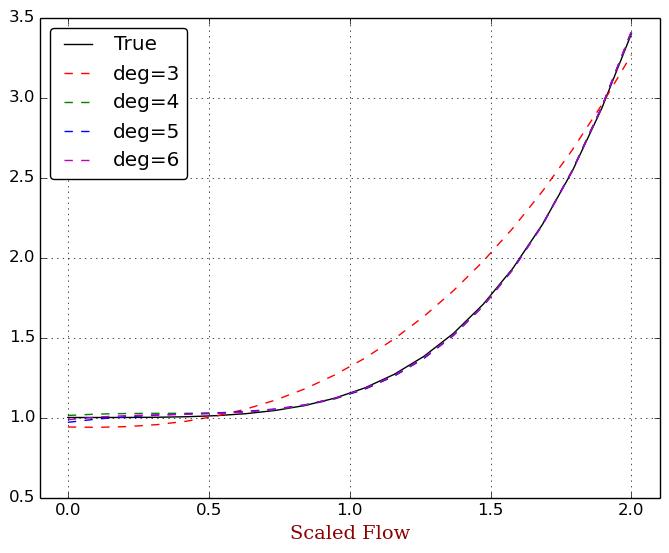
\includegraphics[max size={\textwidth}{\textheight}]{InverseVI_uni_files/InverseVI_uni_16_1.png}
    \par
    \end{center}
    
            \end{InvisibleVerbatim}
            
        
    


    % Make sure that atleast 4 lines are below the HR
    \needspace{4\baselineskip}

    
        \vspace{6pt}
        \makebox[0.1\linewidth]{\smaller\hfill\tt\color{nbframe-in-prompt}In\hspace{4pt}{[}{]}:\hspace{4pt}}\\*
        \vspace{-2.65\baselineskip}
        \begin{ColorVerbatim}
            \vspace{-0.7\baselineskip}
            \begin{Verbatim}[commandchars=\\\{\}]

\end{Verbatim}

            
                \vspace{0.3\baselineskip}
            
        \end{ColorVerbatim}
    

        

        \renewcommand{\indexname}{Index}
        \printindex

    % End of document
    \end{document}


